%&TeX spellcheck = it_IT
\documentclass[12pt,a4paper,twoside]{report}
\usepackage{geometry}%to cus­tomize page lay­out
\usepackage[italian]{babel}%man­ages cul­tur­ally-de­ter­mined ty­po­graph­i­cal (and other) rules, and hy­phen­ation pat­terns
\usepackage[T1]{fontenc}%perchè faccia per bene i caratteri accentati nell'output
\usepackage[utf8]{inputenc}%perchè riconosca i caratteri accentati nel sorgente tex
\usepackage[hyphens]{url}%per inserire url
\usepackage{fancyhdr}%per header e foooter
\usepackage{graphicx}%per le immagini
\usepackage{wrapfig}%to wrap images with text
%\usepackage{epsfig}
\usepackage{amsthm}
\usepackage{listings}%per inserie codice sorgente
\usepackage{xcolor}%colori! :D
\usepackage{amsmath}%per formule matematiche
\usepackage{amssymb} %simboli matematici
\usepackage{booktabs}%en­hances the qual­ity of ta­bles
\usepackage{caption}%to cus­tomise the cap­tions in float­ing en­vi­ron­ments like fig­ure and ta­ble
\usepackage{subfig}%manipulation and ref­er­ence of small or ‘sub’ fig­ures and ta­bles within a sin­gle fig­ure or ta­ble en­vi­ron­ment
\usepackage{eurosym}%The Euro­pean cur­rency sym­bol for the Euro
\usepackage{siunitx}%tante cose sulle unità di misura
\usepackage{calligra}%cal­li­graphic font
\usepackage{verbatim}
\usepackage{indentfirst}%Indent first paragraph after section header
\usepackage{microtype}%fa diventare i font più belli
\usepackage{lmodern}%fontbelli
\usepackage{braket}%parentesi
\usepackage{mathtools}%to en­hance the ap­pear­ance of doc­u­ments con­tain­ing a lot of math­e­mat­ics
\usepackage{mathrsfs}  %per fare le lettere calligrafiche
\usepackage{bm}%define \bm{} that makes the argument bold
\usepackage{empheq}%markup per le formule di amsmath
\usepackage{pstricks}%macros for gen­er­at­ing PostScript that is us­able with most TeX macro for­mats
\usepackage{emptypage}%toglie il numero di pagina alle pahine create con clearpage e cleardoublepage
\usepackage{todonotes}
\usepackage{textcomp}%per il simbolo dei gradi
\usepackage{enumitem}%per controllare gli spazi nelle liste
\usepackage{pbox}%per fare celle con più linee nelle tabelle
\usepackage{placeins}%con \FloatBarrier mette il testo dopo le cose float
\usepackage{longtable}%per tabelle che vanno da una pagina all'altra
\usepackage[final]{pdfpages}%per importare pdf
\usepackage{tkz-graph}


%fine pacchetti

%:::::::::::::::::::::IMPOSTAZIONI::::::::::::::::::::::::::::::::::::::::::::::::::::::::::::::::::::

\geometry{a4paper,top=85pt,bottom=85pt,left=127pt,right=127pt} %imposto la geometria del documento
\captionsetup{tableposition=top,figureposition=bottom,font=small}  %impostazione dei caption di immagini e tabelle
%\DeclareCaptionFormat{elaborazione}{#1#2#3\par}

%::::::::::::::::::::::::::::::::::::::::::::::::::::::::::::::::::::::::::::::::::::::::::::::::::::


\begin{document}

%::::::::::::::::::::::::::DEFINIZIONI DI COMANDI::::::::::::::::::::::::::::::::::::::::::::::::::::
\newcommand{\whitePage}{\cleardoublepage} % pagina bianca e rende la successiva una pagina destra

\newcommand{\HRule}{\rule{\linewidth}{0.6mm}} % command for the horizontal lines, change thickness here

\newcommand*{\eupgrave}{\MakeUppercase{è}} % maiuscola è accentata
%fine comandi
%::::::::::::::::::::::::::::::::::::::::::::::::::::::::::::::::::::::::::::::::::::::::::::::::::::



%::::::::::::::::::::::::::IMPOSTAZIONI GLOBALI::::::::::::::::::::::::::::::::::::::::::::::::::::::
% \setlist(nosep)
%::::::::::::::::::::::::::::::::::::::::::::::::::::::::::::::::::::::::::::::::::::::::::::::::::::


%::::::::::::::::::::::::::::::::TITLE PAGE::::::::::::::::::::::::::::::::::::::::::::::::::::::::::
\begin{titlepage}



\center  % Center everything on the page

\textsc{\Large \\[4.5cm]Università degli Studi di Padova}\\[1.5cm]
\textsc{\Large Corso di laurea triennale in Ingegneria dell'Informazione}\\[0.5cm]

\noindent\rule{\textwidth}{0.6pt}\\[0.4cm]
{ \Large{\bfseries Analisi di una rete di autori di pubblicazioni scientifiche}}\\[0.4cm]
\noindent\rule{\textwidth}{0.6pt}\\[1cm]


\includegraphics[height=4cm]{img/unipd-bn}\\[1cm]


\begin{minipage}{0.4\textwidth}
\begin{flushleft} \large
\emph{Laureando:}\\
Pietro Maria \textsc{Nobili} % Your name
\end{flushleft}
\begin{flushleft} \large
\emph{Matricola:}\\
1067941 % Your number
\end{flushleft}
\end{minipage}
~
\begin{minipage}{0.5\textwidth}
\begin{flushright} \large
\emph{Relatore:} \\
Prof.ssa Cinzia \textsc{Pizzi} \\% Supervisor's Name
\end{flushright}
\begin{flushright} \large
\emph{Correlatore:} \\
Dott. Mattia \textsc{Samory} % Supervisor's Name
\end{flushright}
\end{minipage}\\[2cm]


{\large 18 Luglio 2018}\\
{\large Anno Accademico 2017/2018}\\[3cm] % Date, change the \today to a set date if you want to be precise


\vfill % Fill the rest of the page with whitespace

\end{titlepage}
%::::::::::::::::::::::::::::::::::::::::::::::::::::::::::::::::::::::::::::::::::::::::::::::::::::


\whitePage

%::::::::::::::::::::::::::::::::::INDEX:::::::::::::::::::::::::::::::::::::::::::::::::::::::::::::

\pagenumbering{Roman}
\tableofcontents

%::::::::::::::::::::::::::::::::::::::::::::::::::::::::::::::::::::::::::::::::::::::::::::::::::::



%::::::::::::::::::::::::::::::::::THE REAL CONTENT::::::::::::::::::::::::::::::::::::::::::::::::::

\whitePage



\newpage
\pagenumbering{arabic}
\setcounter{page}{1}
\section*{Abstract} \label{abstract} % the asterisk is to remove the numbering
\addcontentsline{toc}{chapter}{Abstract} % we put the asterisk so we add it manually to the toc
% qua ci sarà un glorioso abstract
È stato generato un grafo delle pubblicazioni del DEI.

Sono stati cercati cluster nel grafo.

% TODO spezzettare le parole in un abstract è orribile
Sono stati confrontati con la struttura delle comunità del dipartimento.


% \whitePage
\section*{Introduzione} \label{introduzione}
\addcontentsline{toc}{chapter}{Introduzione} % we put the asterisk so we add it manually to the toc

Breve descrizione del community detection e della sua importanza, in generale e nel caso particolare
delle comunità di autori di pubblicazioni scientifiche.

Presentazione della struttura della tesi.



\whitePage
\chapter{Community detection} \label{cap:comdet}

\section{Studi precedenti} \label{sec:storia}
Descrizione della community detection.

Descrizione della bibliografia attuale sui grafi di coautori.

\section{Metodi usati} \label{sec:metodi}
Che metodi vengono usati per generare le comunità.

\subsection{Girvan–Newman} \label{subsec:gn}
Descrizione metodo GN.

Nella libreria SNAP di Stanford \cite{snapnets}

\subsection{Blockmodel} \label{subsec:bn}
Descrizione metodo blockmodel.

\subsection{Clauset-Newman-Moore} \label{subsec:cnm}
Descrizione metodo Clauset-Newman-Moore.

\subsection{Louvain} \label{subsec:lou}
Descrizione metodo Louvain se implementato.



\whitePage
\chapter{Estrazione dati} \label{cap:estrazione}

\section{Struttura database Microsoft} \label{sec:msr}
% https://academic.microsoft.com/#/faq https://dl.acm.org/citation.cfm?doid=2740908.2742839 citato
% da qua
Il database da cui sono stati estratti i dati è il Microsoft Academic Graph
\cite{Sinha:2015:OMA:2740908.2742839}, che contiene informazioni relative a pubblicazioni
scientifiche, autori, istituzioni accademiche, riviste, conferenze e settori di studio. I record
presenti nei file forniscono le relazioni tra queste entità.

Il database è composto da undici file di testo che contengono un record per riga, con i campi
separati da tabulazione.

Per il lavoro oggetto di questa tesi sono stati utilizzati in particolare quattro file del database,
la cui struttura è illustrata nella tabella \ref{table:msrstruttura1}.

L'ultimo aggiornamento del database disponibile risale all'agosto 2015.
\begin{center}
%\begin{table}
%\begin{tabular}{| l | l |}
\captionof{table}{Struttura del database}
\label{table:msrstruttura1}
\begin{longtable}{| l | l |}
\hline
Nome file&
Campi\\
(Numero record)&\\
\hline
Authors.txt&Author ID\\
(123.017.489)&Author Name\\
\hline
PaperAuthorAffiliations.txt&Paper ID\\
(325.498.063)&Author ID\\
&Affiliation ID\\
&Original affiliation name\\
&Normalized affiliation name\\
&Author sequence number\\
\hline
Affiliations.txt&Affiliation ID\\
(2.719.436)&Affiliation name\\
\hline
Papers.txt&Paper ID\\
(122.695.085)&Original paper title\\
&Normalized paper title\\
&Paper publish year\\
&Paper publish date\\
&Paper Document Object Identifier (DOI)\\
&Original venue name\\
&Normalized venue name\\
&Journal ID mapped to venue name\\
&Conference series ID mapped to venue name\\
&Paper rank\\
\hline
%\end{tabular}
%\caption{Struttura del database}
%\label{table:msrstruttura}
\end{longtable}
%\end{table}
\end{center}
\FloatBarrier

\section{Processo di estrazione} \label{sec:processo}
%\subsection{Approccio iniziale} \label{subsec:primo}
Dal sito di dipartimento (\url{http://www.dei.unipd.it/lista-docenti}) sono stati estratti i nomi
degli attuali afferenti DEI, includendo Docenti, Assegnisti di ricerca, Collaboratori di ricerca e
Dottorandi.

La lista ottenuta comprende 379 autori.
% TODO non fare il pezzente e scrivi quanti hanno l'etichetta
Dove presente, è stato estratto il Settore Scientifico Disciplinare dell'afferente, che ha fornito
la partizione in classi utilizzata come rifermento alla fine dell'elaborazione dei dati.

I nomi propri degli autori sono stati abbreviati in tutte le possibili combinazioni per rispecchiare
la struttura del database Microsoft, ed è stato creato un file con la struttura seguente:

\begin{center}
\captionof{table}{PersoneComunitaDEI.txt}
\begin{minipage}{0.90\textwidth}
\begin{verbatim}
a a pietracaprina            INF/01 - INFORMATICA
a alberto pietracaprina	     INF/01 - INFORMATICA
andrea a pietracaprina	      INF/01 - INFORMATICA
andrea alberto pietracaprina	INF/01 - INFORMATICA
...

\end{verbatim}
\end{minipage}
\end{center}

Utilizzando questa lista di nomi ed abbreviazioni, sono stati estratti dal file \textit{Authors.txt}
le coppie (ID autore, nome autore), che risultano essere 8.135, con una media di 21,5 ID per nome.

Con il set di ID autori ottenuto, sono stati estratti dal file \textit{PaperAuthorAffiliations.txt}
i record relativi ai paper, nella forma (ID paper, ID autore, ID affiliation), per un totale di
62.291 paper.

Dalla lista così ottenuta, non necessariamente ordinata, sono stati creati gli edge fra ID autore,
che sono poi stati aggregati creando una edge list pesata, come indicato in \ref{tab:creazioneedge}

\begin{center}

% TODO mettere caption degli esempietti senza tabella
%\captionof{elaborazione}{Creazione edge}
%Creazione edge
\captionof{table}{Creazione edge}
\label{tab:creazioneedge}
\begin{minipage}{0.40\textwidth}
\begin{verbatim}
IDpaper1  IDautore1
IDpaper1  IDautore2
IDpaper1  IDautore3
IDpaper2  IDautore2
IDpaper2  IDautore3
\end{verbatim}
\end{minipage}
\begin{minipage}{0.075\textwidth}
$\rightarrow$
\end{minipage}
\begin{minipage}{0.40\textwidth}
\begin{verbatim}
IDautore1  IDautore2  1
IDautore1  IDautore3  1
IDautore2  IDautore3  2
\end{verbatim}
\end{minipage}
\end{center}
A partire da questi edge è stato generato il primo grafo che rappresenta la rete degli autori.
% TODO riscrivila

Questo metodo di creazione del grafo, che considera le collaborazioni tra autori, riduce a 778 il
set di ID autori per un totale di 287 nomi univoci. Il grafo è formato da 1.830 edge con 7.803 di
peso totale.

I grafi in questo capitolo sono stati divisi in comunità utilizzando l'algoritmo Modularity di
Gephi.


\centerline{
\begin{minipage}{1.45\textwidth}
\setlength{\fboxrule}{0pt}	%barbatrucco per far sparire il bordo della box
\fbox{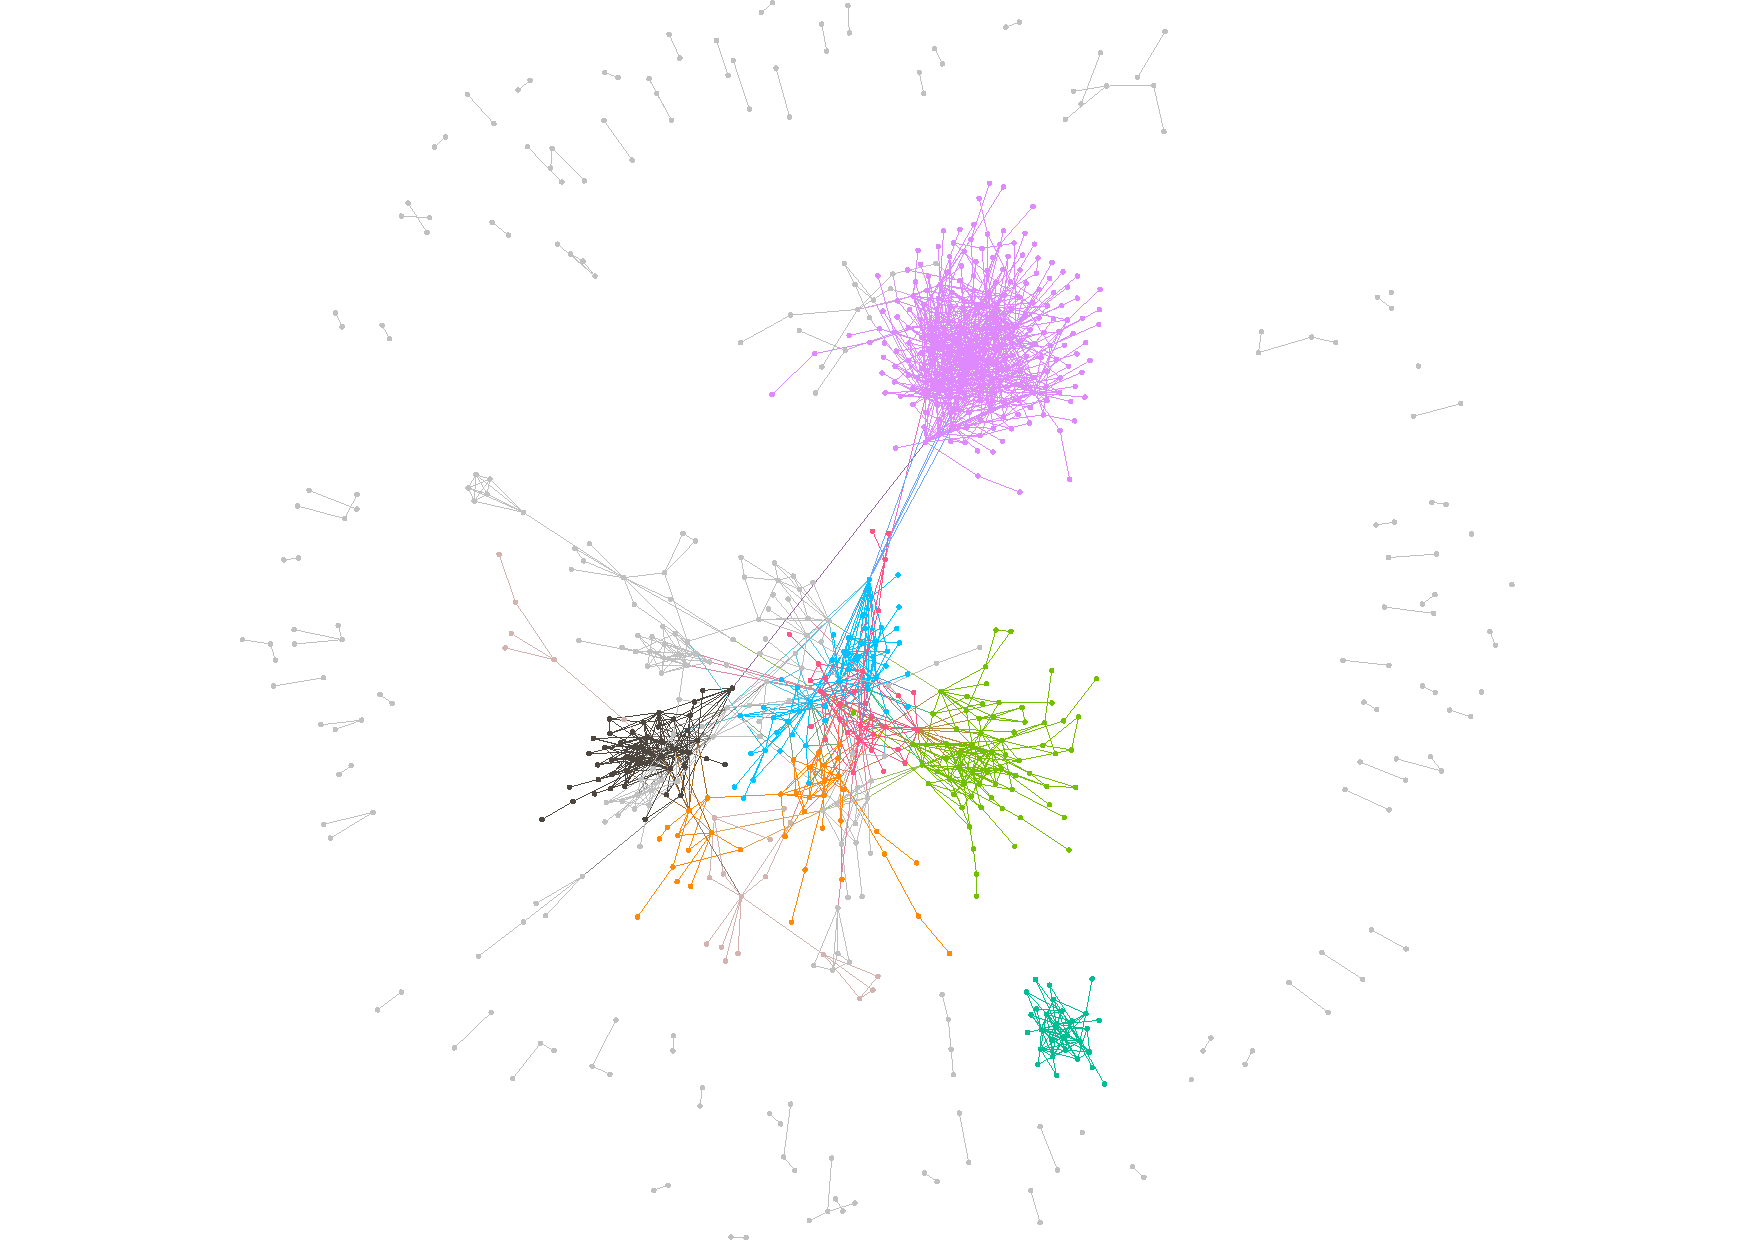
\includegraphics[page=1,scale=0.60]{img/GrafoCollaborazioni.pdf}}
\captionof{figure}{Grafo collaborazioni}
\label{img:grafotutti}
\end{minipage}
}

%\begin{minipage}{1.4\textwidth}
%%[width=\textwidth]
%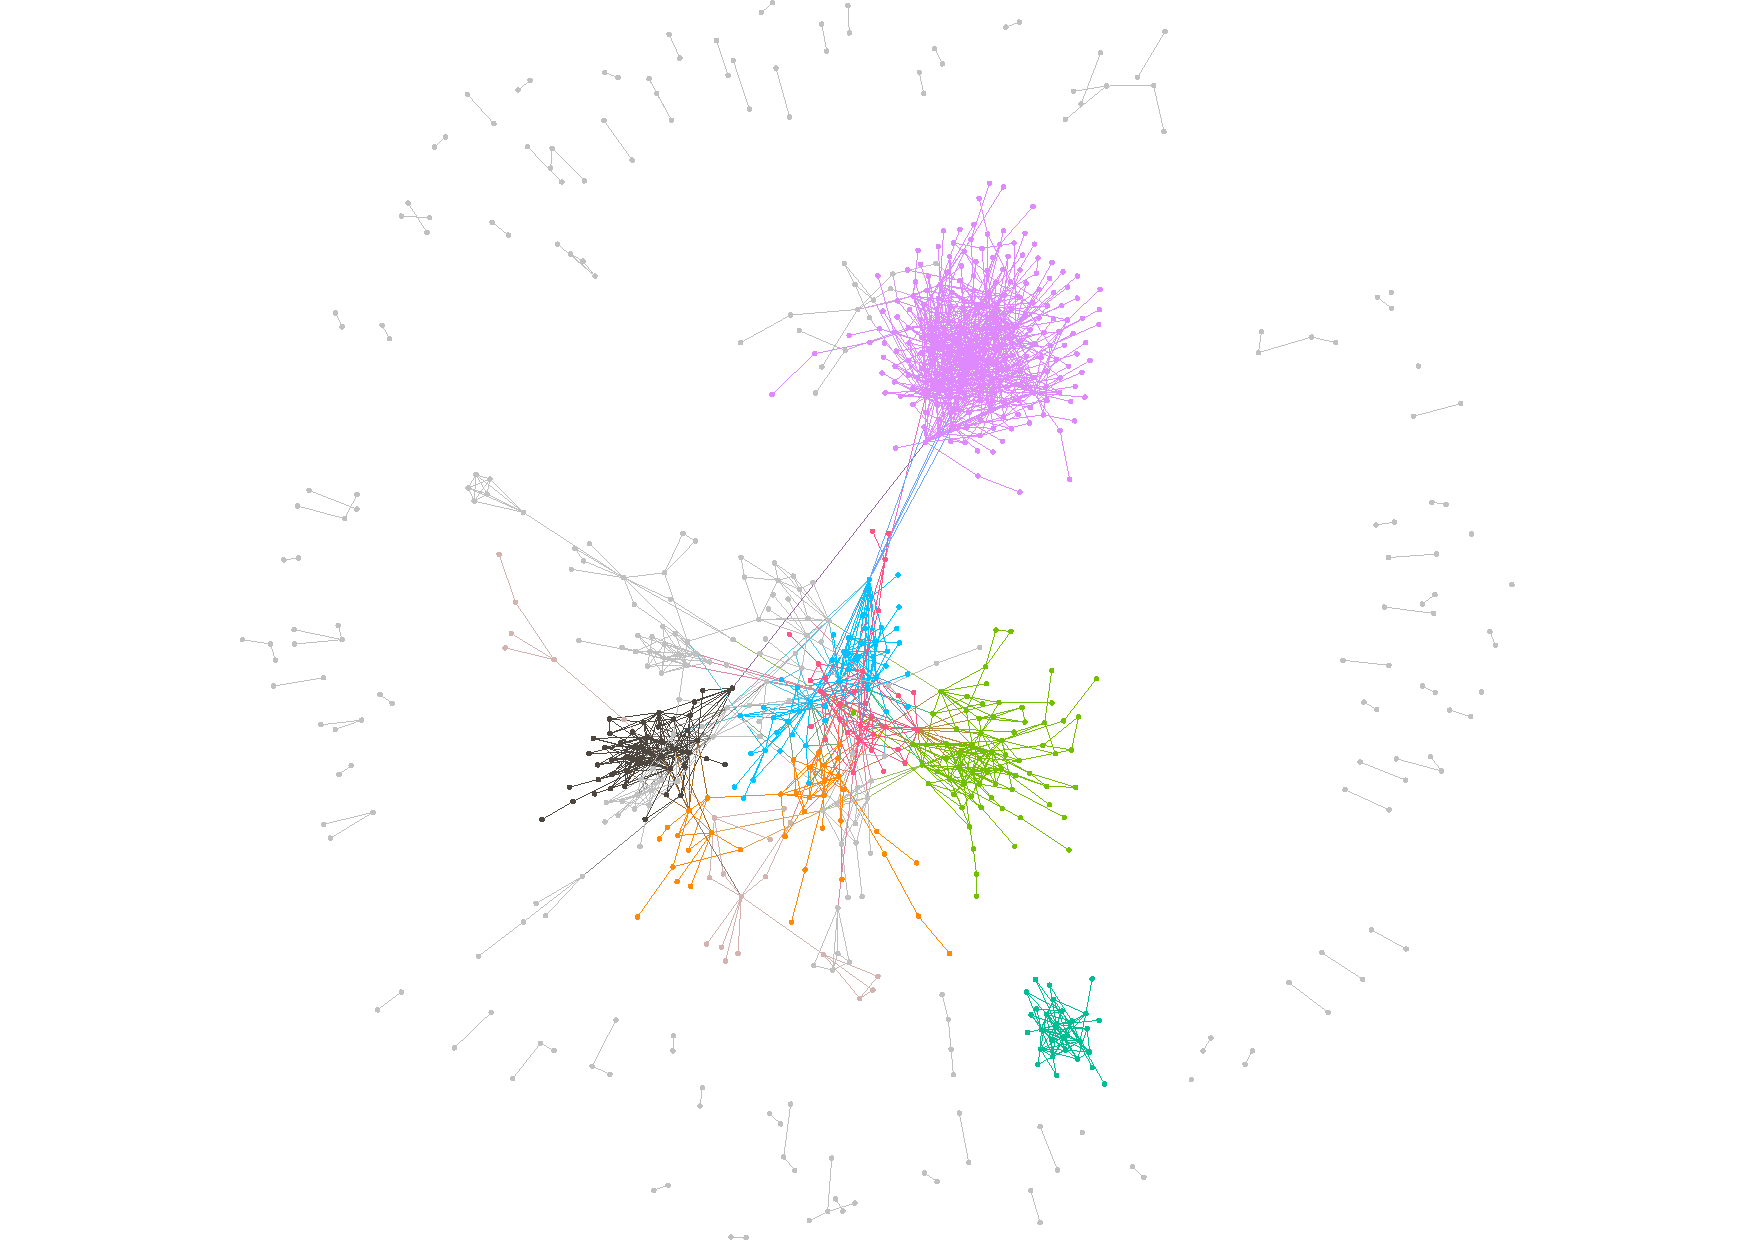
\includepdf{img/GrafoCollaborazioni.pdf}
%\captionof{figure}{Grafo collaborazioni}
%\label{img:grafoprimo}
%\end{minipage}
%\clearpage

\subsubsection{Analisi della prima estrazione}\label{ssc:analisiuno}

I due problemi principali di questo processo emergono al momento dell'estrazione degli ID autore dal
file \textit{Authors.txt}:

\begin{itemize}[noitemsep, topsep=0pt]
\item
Vengono selezionati anche gli ID riferiti ad autori omonimi, non affiliati al DEI.
\item
Ad un singolo autore DEI sono associati più ID autore.
\end{itemize}

%::::PADOVANI::::
\subsection{Filtro degli autori per affiliation} \label{ssc:padovani}
Il primo problema è già in parte risolto dal metodo di creazione del grafo, che considera solo gli
ID autori che hanno almeno una collaborazione con un altro ID nel set. In questo modo più del 90\%
degli ID viene filtrato.

È stato sviluppato un secondo metodo di estrazione dei dati che esclude gli ID autore se non hanno
mai pubblicato un paper a Padova, considerando le informazioni sulle affiliation dei paper, come
viene illustrato di seguito.

\begin{itemize}[noitemsep, topsep=0pt]
\item[--]
Dal file \textit{Affiliations.txt} si estrae la lista delle affiliation in cui risulta nel nome un match all'espressione regolare ``$pad(ov|u)a$''.
% TODO usare un set di affiliation solo di dipartimento (circa 300) è troppo poco
\item[--]
% TODO richiamare la lista di terne
Dalla lista di terne (ID paper, ID autore, ID affiliation) si mantengono solo quelle in cui l'ID affiliation compare nel set di affiliation padovane appena estratte.
\item[--]
Dalle terne selezionate, si estrae un set di ID autori che hanno pubblicato almeno un paper con affiliation padovana.
\item[--] % TODO meglio - più punti
Si estraggono i paper scritti da questi ID autore e si procede alla generazione degli edge pesati.
\end{itemize}

Applicando questo metodo, gli ID autore si riducono a 306, relativi a 201 nomi univoci. Il grafo generato include 850 edge con un peso totale di 5.195.

\centerline{
\begin{minipage}{1.10\textwidth}
\setlength{\fboxrule}{0pt}	%barbatrucco per far sparire il bordo della box
\fbox{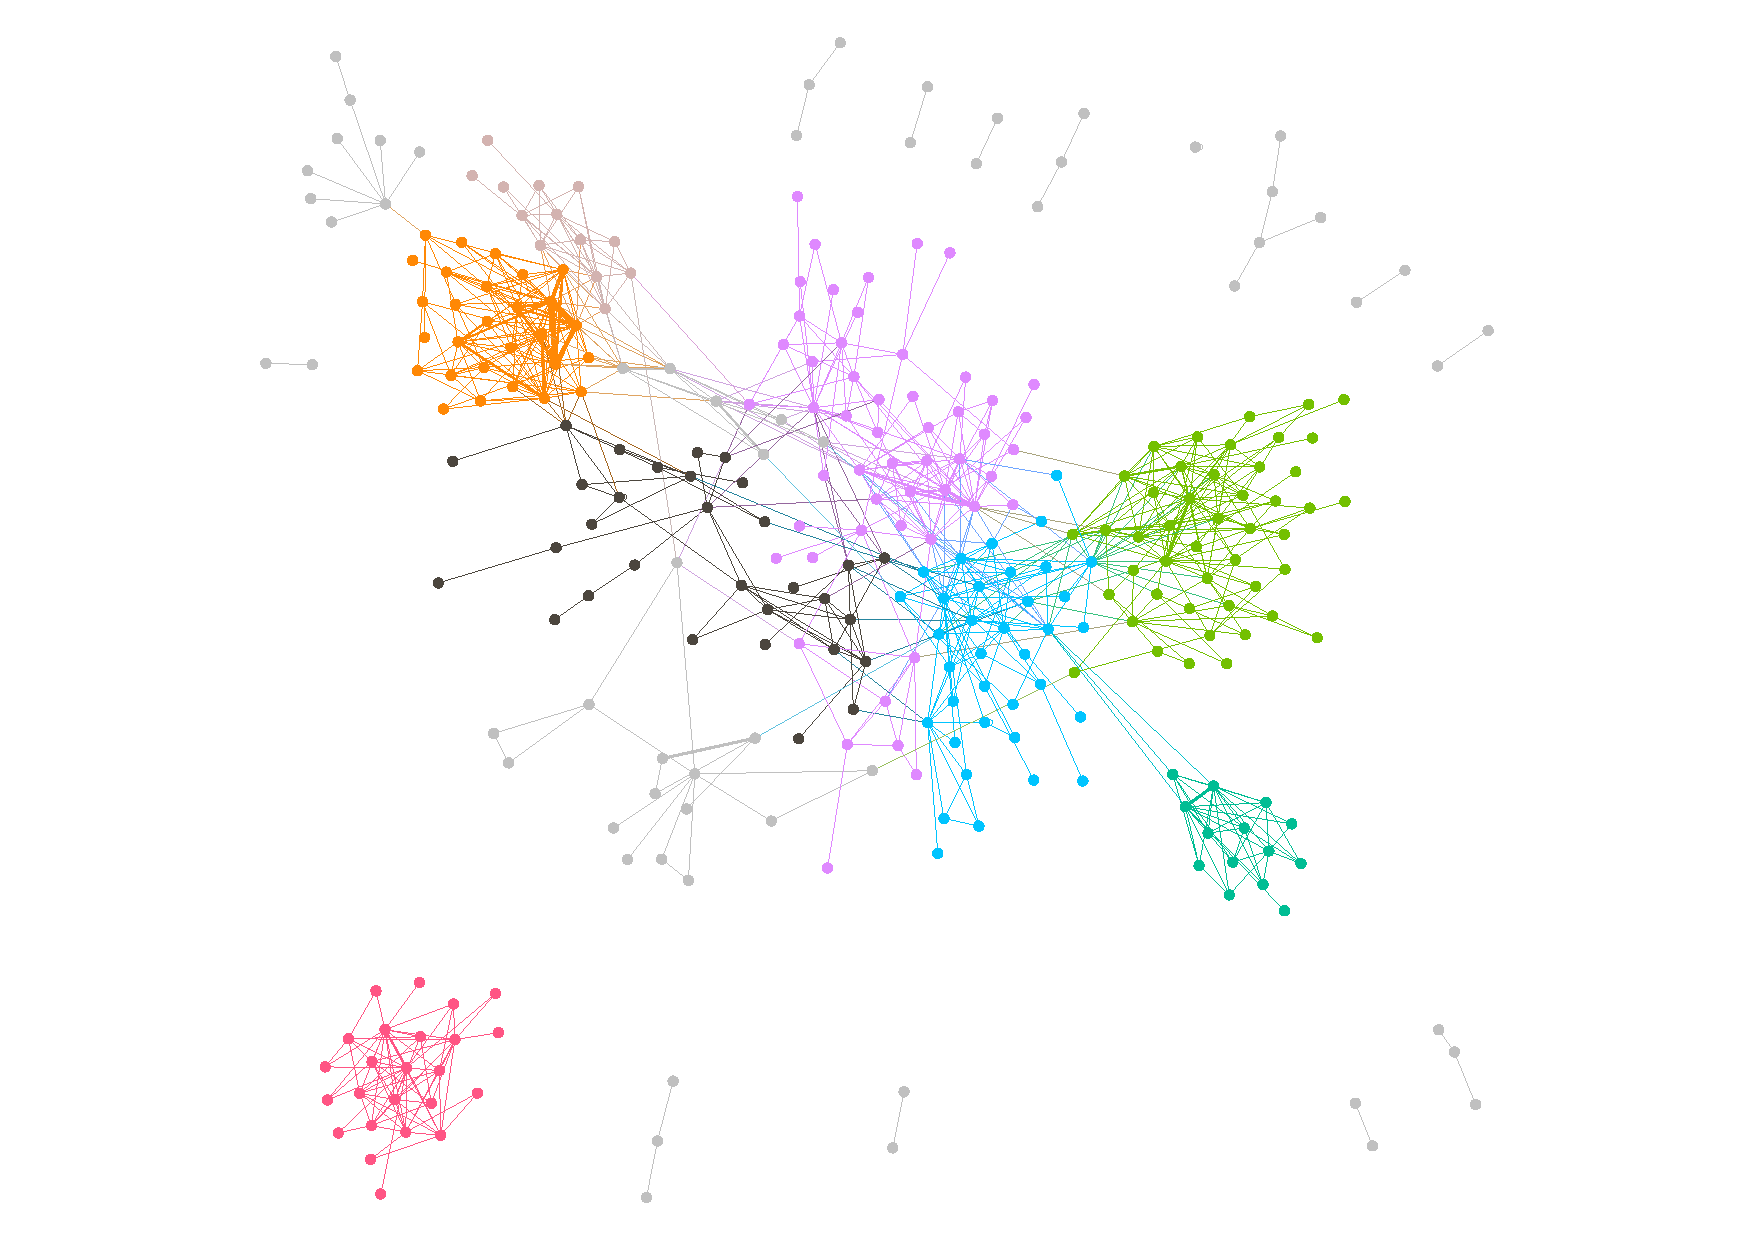
\includegraphics[page=1,scale=0.45]{img/GrafoPadovani.pdf}}
\captionof{figure}{Grafo Padovani}
\label{img:grafopad}
\end{minipage}
}

%::::::::::::::::::::::::::::::::::COLLASSANODI::::::::::::::::::::::::::::::::::::::::::::::::::::::
\subsection{Unione di ID autore in singoli nodi} \label{ssc:collassa}
% TODO esempio di qualcuno
Per risolvere il secondo problema insorto nell'estrazione dei dati, per cui ad una singola persona
fisica, effettivamente affiliata al DEI, possono essere associati più ID autore, sono state seguite
due vie alternative fra loro.

Il primo metodo tiene conto solo dei nomi associati ai nodi del grafo, il secondo metodo sfrutta la
struttura del grafo per stabilire se due nodi siano riferiti alla stessa persona.

% I grafi precedentemente generati vengono rielaborati

\subsubsection{Per nome} \label{ssc:nomi} % questo label è inutile

I grafi precedentemente generati vengono rielaborati, ipotizzando che nodi con nomi uguali o le cui
abbreviazioni sono uguali possano essere considerati un unico nodo.

In questo modo ``\textit{a alberto pietracaprina}'' viene associato a ``\textit{a a
pietracaprina}'' ma anche a ``\textit{andrea a pietracaprina}'' come pure a ``\textit{andrea alberto
pietracaprina}''.

I nodi del grafo in figura \ref{img:grafotutti} si riducono da 778 a 199. Gli edge scendono da 1830
a 661, mantenendo lo stesso peso totale di 7.803.

\centerline{
\begin{minipage}{1.10\textwidth}
\setlength{\fboxrule}{0pt}	%barbatrucco per far sparire il bordo della box
\fbox{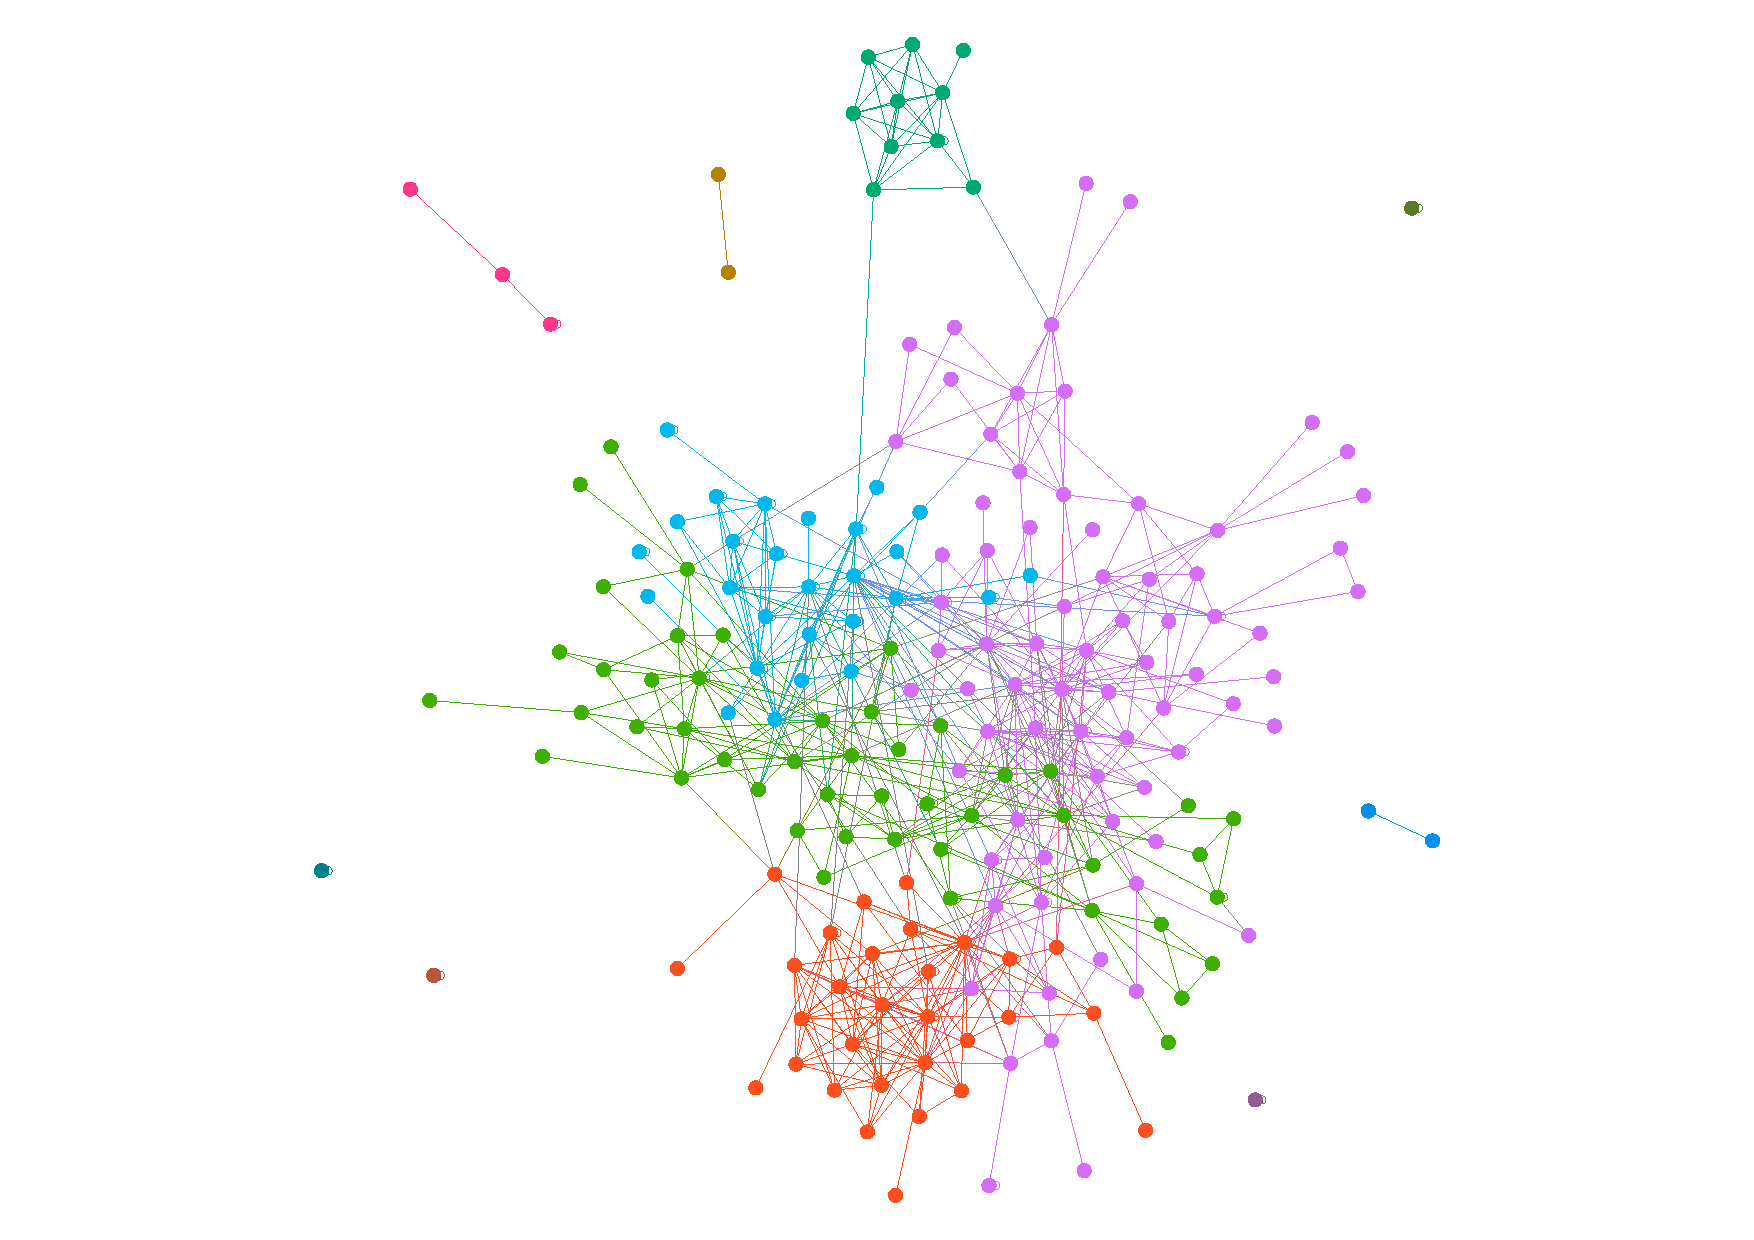
\includegraphics[page=1,scale=0.37]{img/GrafoTuttiNomi.pdf}}
\captionof{figure}{Grafo collaborazioni - nodi unificati per nome}
\label{img:grafotuttinome}
\end{minipage}
}

\clearpage % grafica da fare alla fine
I nodi del grafo in figura \ref{img:grafopad} si riducono da 306 a 158. Gli edge scendono da 850 a
463, mantenendo il peso totale di 5.195.

\centerline{
\begin{minipage}{1.10\textwidth}
\setlength{\fboxrule}{0pt}	%barbatrucco per far sparire il bordo della box
\fbox{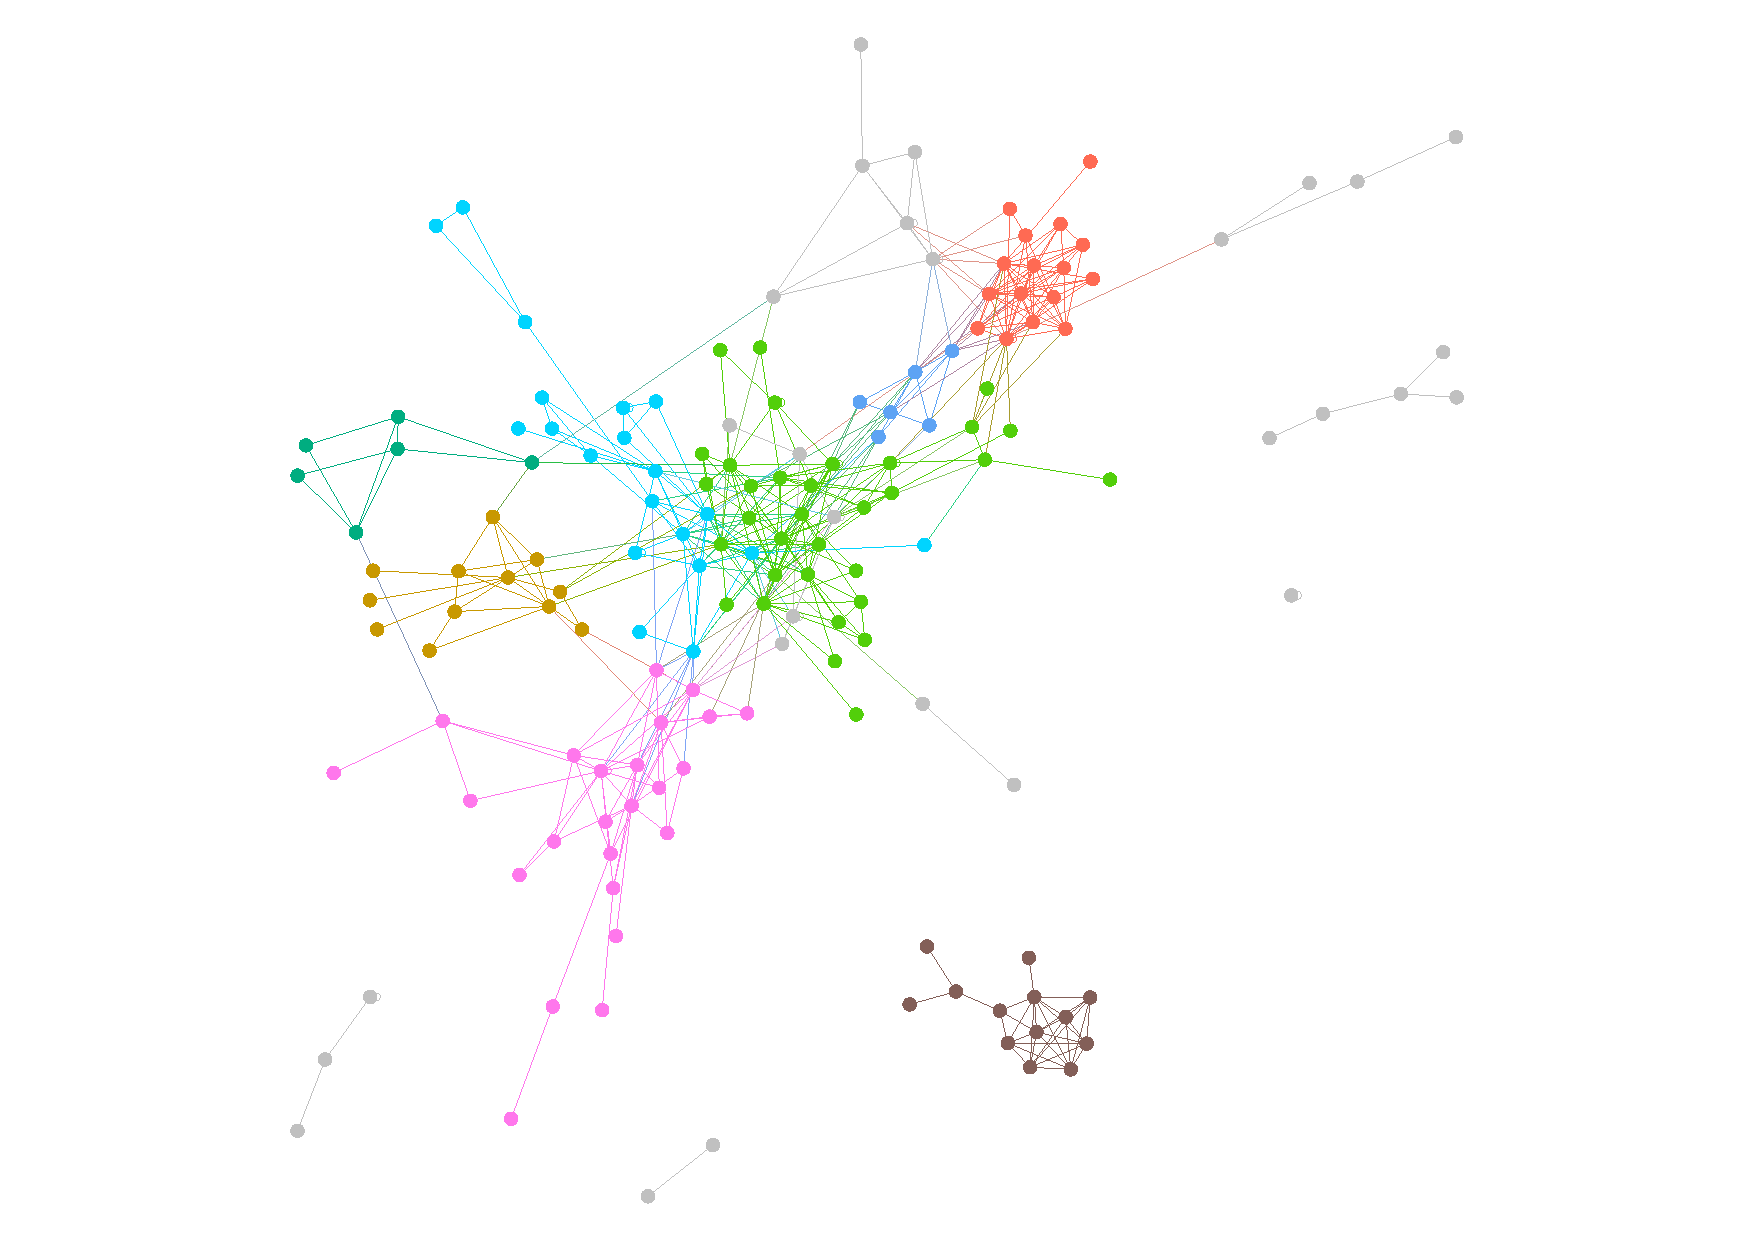
\includegraphics[page=1,scale=0.37]{img/GrafoPadovaniNomi.pdf}}
\captionof{figure}{Grafo padovani - nodi unificati per nome}
\label{img:grafopadnome}
\end{minipage}
}

\subsubsection{Per distanza} \label{ssc:distanza}

Il metodo che considera i nomi precedentemente descritto introduce una criticità nel caso un cui due
autori abbiano un nome che viene abbreviato nello stesso modo.
Questo fa sì che più persone vengano assimilate erroneamente in un unico nodo.

Nei dati che sono stati trattati questo succede solo nel caso di ``\textit{Mattia Zorzi}'' e
``\textit{Michele Zorzi}'', che si abbreviano entrambi in ``\textit{m zorzi}''.

In dataset più ampi oppure relativi a comunità che anche se ristrette presentano una bassa
variabilità dei cognomi, il fenomeno dei falsi positivi incide in maniera molto più marcata sulla
veridicità del grafo.

Nel secondo metodo sviluppato per unificare i nodi, viene richiesta un'ulteriore condizione per
considerare due nodi come relativi alla stessa persona fisica. Oltre a verificare la corrispondenza
delle abbreviazioni dei nomi si calcola anche la distanza minima tra i due nodi nel grafo. Se questa
distanza è minore di una certa soglia, i due nodi vengono unificati. Questo processo può essere
iterato più volte, per sfruttare le informazioni ottenute nei passi precedenti.

\clearpage % grafica da fare alla fine
\begin{center}
\captionof*{table}{Prima iterazione unione nodi con distanza minima minore di 2}
\begin{minipage}{0.40\textwidth}
\begin{tikzpicture}
\GraphInit[vstyle=Normal]
%\draw[help lines] (0,0) grid (4,3);
\Vertex[L=D]{d1} % par défaut x = 0 et y = 0
\Vertex[x=1 , y=1.5, L=A]{a2}
\Vertex[x=0 , y=3, L=C]{c1}
\Vertex[x=2 , y=0, L=A]{a1}
\Vertex[x=2 , y=3, L=B]{b1}
\Vertex[x=3 , y=1.5, L=A]{a3}
\Vertex[x=4 , y=3, L=C]{c2}
\Edge[label=3](c1)(a2)
\Edge[label=8](a3)(c2)
\SetUpEdge[style={ultra thick},color=red]
\Edge[label=6](d1)(a1)
\Edge[label=7](d1)(a2)
\SetUpEdge[style={ultra thick},color=cyan]
\Edge[label=1](a2)(b1)
\Edge[label=2](b1)(a3)
\end{tikzpicture}
\end{minipage}
\begin{minipage}{0.075\textwidth}
$\rightarrow$
\end{minipage}
\begin{minipage}{0.40\textwidth}
\begin{tikzpicture}
\GraphInit[vstyle=Normal]
\Vertex[L=D]{d1} % par défaut x = 0 et y = 0
\Vertex[x=2 , y=1.5, L=A]{a2}
\Vertex[x=0 , y=3, L=C]{c1}
\Vertex[x=2 , y=3, L=B]{b1}
\Vertex[x=4 , y=3, L=C]{c2}
\Edge[label=13](d1)(a2)
\Edge[label=3](a2)(b1)
\Edge[label=3](c1)(a2)
\Edge[label=8](a2)(c2)
\end{tikzpicture}
\end{minipage}
\end{center}

\begin{center}
\captionof*{table}{Seconda iterazione unione nodi con distanza minima minore di 2}
\begin{minipage}{0.40\textwidth}
\begin{tikzpicture}
\GraphInit[vstyle=Normal]
\Vertex[L=D]{d1} % par défaut x = 0 et y = 0
\Vertex[x=2 , y=1.5, L=A]{a2}
\Vertex[x=0 , y=3, L=C]{c1}
\Vertex[x=2 , y=3, L=B]{b1}
\Vertex[x=4 , y=3, L=C]{c2}
\Edge[label=13](d1)(a2)
\Edge[label=3](a2)(b1)
\SetUpEdge[style={ultra thick},color=orange]
\Edge[label=3](c1)(a2)
\Edge[label=8](a2)(c2)
\end{tikzpicture}
\end{minipage}
\begin{minipage}{0.075\textwidth}
$\rightarrow$
\end{minipage}
\begin{minipage}{0.40\textwidth}
\begin{tikzpicture}
\GraphInit[vstyle=Normal]
\Vertex[L=D]{d1} % par défaut x = 0 et y = 0
\Vertex[x=2 , y=1.5, L=A]{a2}
\Vertex[x=0.8 , y=3, L=C]{c1}
\Vertex[x=3.2 , y=3, L=B]{b1}
\Edge[label=13](d1)(a2)
\Edge[label=11](c1)(a2)
\Edge[label=3](a2)(b1)
\end{tikzpicture}
\end{minipage}
\end{center}

I valori ottimi di soglia e numero di iterazioni sono stati cercati sperimentalmente, ma non è
emersa dai risultati una coppia di valori migliore in maniera rilevante rispetto alle altre.
% TODO riferimento alla spiegazione del perché nel capitolo 4
Ispezionando manualmente il grafo, si è constatato che ID autore riferiti alla stessa persona
risultano generalmente distanti 2. Il procedimento è stato ripetuto tre volte, in modo da sfruttare
le informazioni generate nei passi predecenti. Dopo questo numero di iterazioni il grafo raggiunge
quasi una situazione di stabilità.

\clearpage % grafica da fare alla fine

I nodi del grafo in figura \ref{img:grafotutti} si riducono da 778 a 336. Gli edge scendono da 1830
a 634, mantenendo lo stesso peso totale di 7.803.

\centerline{
\begin{minipage}{1.20\textwidth}
\setlength{\fboxrule}{0pt}	%barbatrucco per far sparire il bordo della box
\fbox{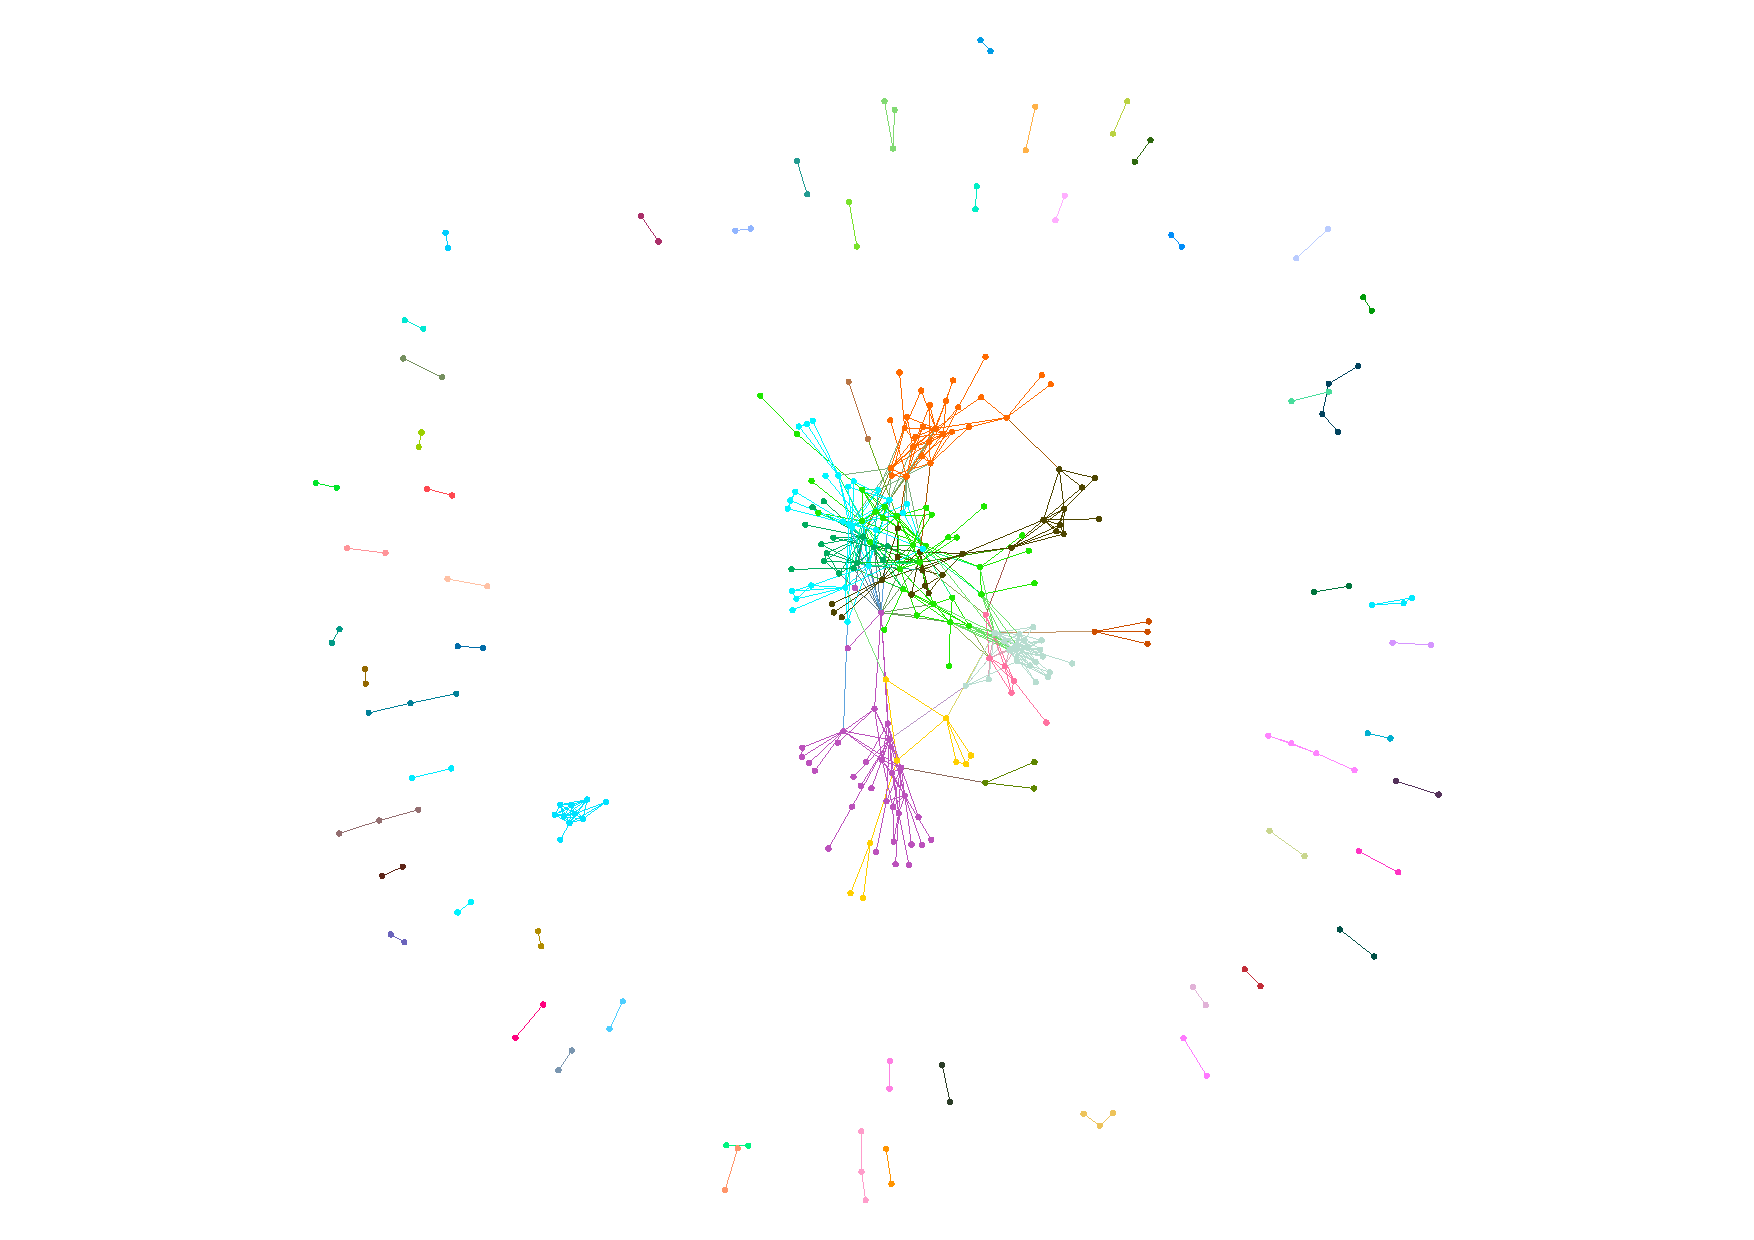
\includegraphics[page=1,scale=0.47]{img/GrafoTuttiDistanza23.pdf}}
\captionof{figure}{Grafo collaborazioni unificati per distanza}
\label{img:grafotuttidistanza}
\end{minipage}
}

I nodi del grafo in figura \ref{img:grafopad} si riducono da 306 a 173. Gli edge scendono da 850 a
439, mantenendo il peso totale di 5.195.

\centerline{
\begin{minipage}{1.00\textwidth}
\setlength{\fboxrule}{0pt}	%barbatrucco per far sparire il bordo della box
\fbox{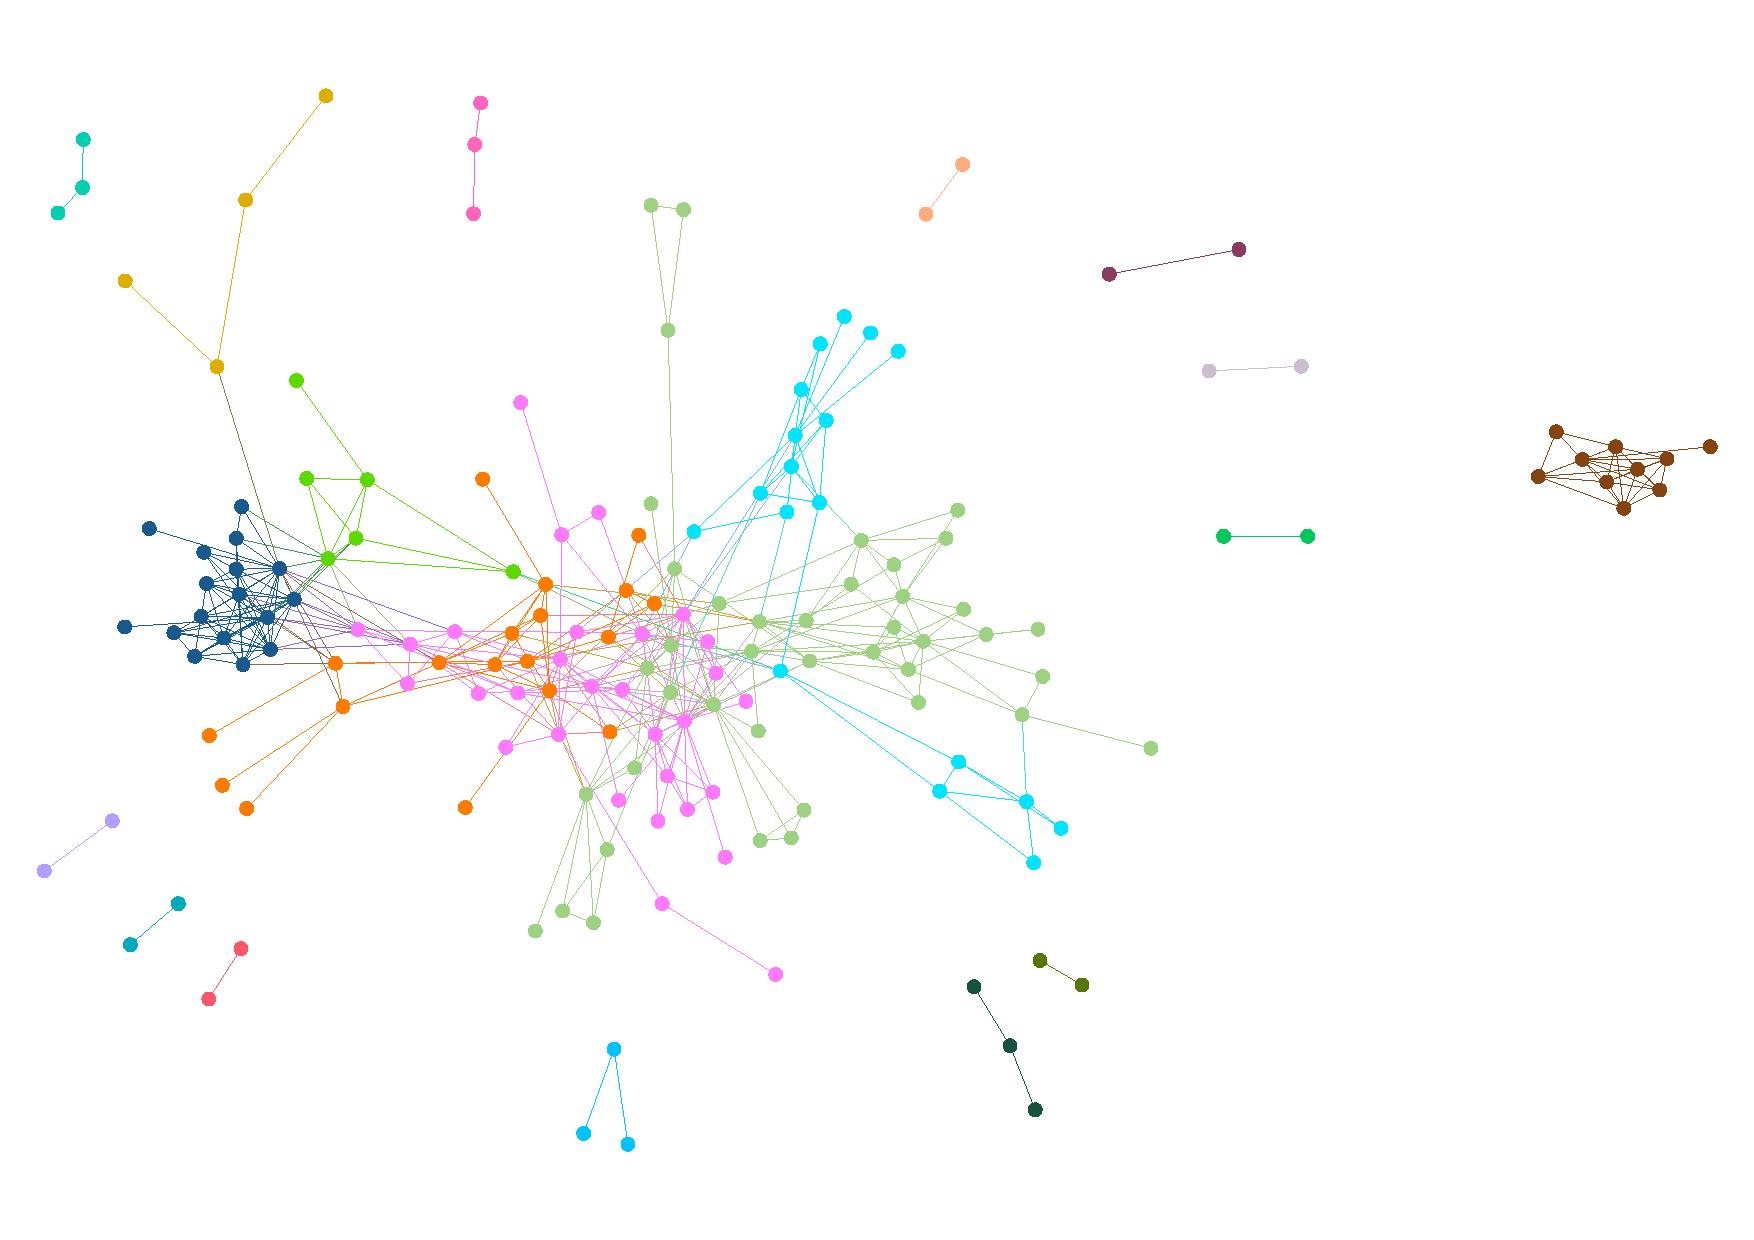
\includegraphics[page=1,scale=0.37]{img/GrafoPadovaniDistanza23.pdf}}
\captionof{figure}{Grafo Padovani unificati per distanza}
\label{img:grafopaddistanza}
\end{minipage}
}

% TODO mostra tabella o grafico dei confronti delle iterazioni varie

\clearpage % grafica da fare alla fine

\subsubsection{Per nodi adiacenti} \label{ssc:edge}
Osservando i grafi generati senza unire i nodi, si nota la presenza di un elevato numero di
componenti sconnesse formate da 2-4 autori, che sono principalmente effettivi collaboratori tra
loro. È stato sviluppato un metodo di deduplicazione dei nodi che si basa sulle collaborazioni tra
coppie di autori.

Per ogni edge si estraggono i nomi relativi agli estremi, se due edge hanno gli estremi con i nomi
coincidenti, si considerano le coppie di nodi come relative alla stessa persona.

\begin{center}
\captionof*{table}{Unione dei nodi per coppie di nodi adiacenti}
\begin{minipage}{0.40\textwidth}
\begin{tikzpicture}
\GraphInit[vstyle=Normal]
\Vertex[L=B]{b1} % par défaut x = 0 et y = 0
\Vertex[x=2 , y=1.5, L=A]{a2}
\Vertex[x=0.5 , y=1.5, L=A]{a1}
\Vertex[x=2.5 , y=3, L=C]{c1}
\Vertex[x=1.5 , y=0, L=B]{b2}
\Vertex[x=4 , y=3, L=C]{c2}
\Edge[label=2](b2)(a2)
\Edge[label=3](a1)(b1)
\Edge[label=4](c1)(a2)
\Edge[label=6](a2)(c2)
\SetUpEdge[style={dashed},color=orange]
\Edge(b1)(b2)
\Edge(a1)(a2)
\Edge(c1)(c2)
\end{tikzpicture}
\end{minipage}
\begin{minipage}{0.075\textwidth}
$\rightarrow$
\end{minipage}
\begin{minipage}{0.40\textwidth}
\begin{tikzpicture}
\GraphInit[vstyle=Normal]
\Vertex[L=B]{b1} % par défaut x = 0 et y = 0
\Vertex[x=2 , y=1.5, L=A]{a2}
\Vertex[x=4 , y=3, L=C]{c1}
\Edge[label=10](c1)(a2)
\Edge[label=5](a2)(b1)
\end{tikzpicture}
\end{minipage}
\end{center}

I nodi del grafo in figura \ref{img:grafotutti} si riducono da 778 a 313. Gli edge scendono da 1830
a 615, mantenendo lo stesso peso totale di 7.803.

\centerline{
\begin{minipage}{1.05\textwidth}
\setlength{\fboxrule}{0pt}	%barbatrucco per far sparire il bordo della box
\fbox{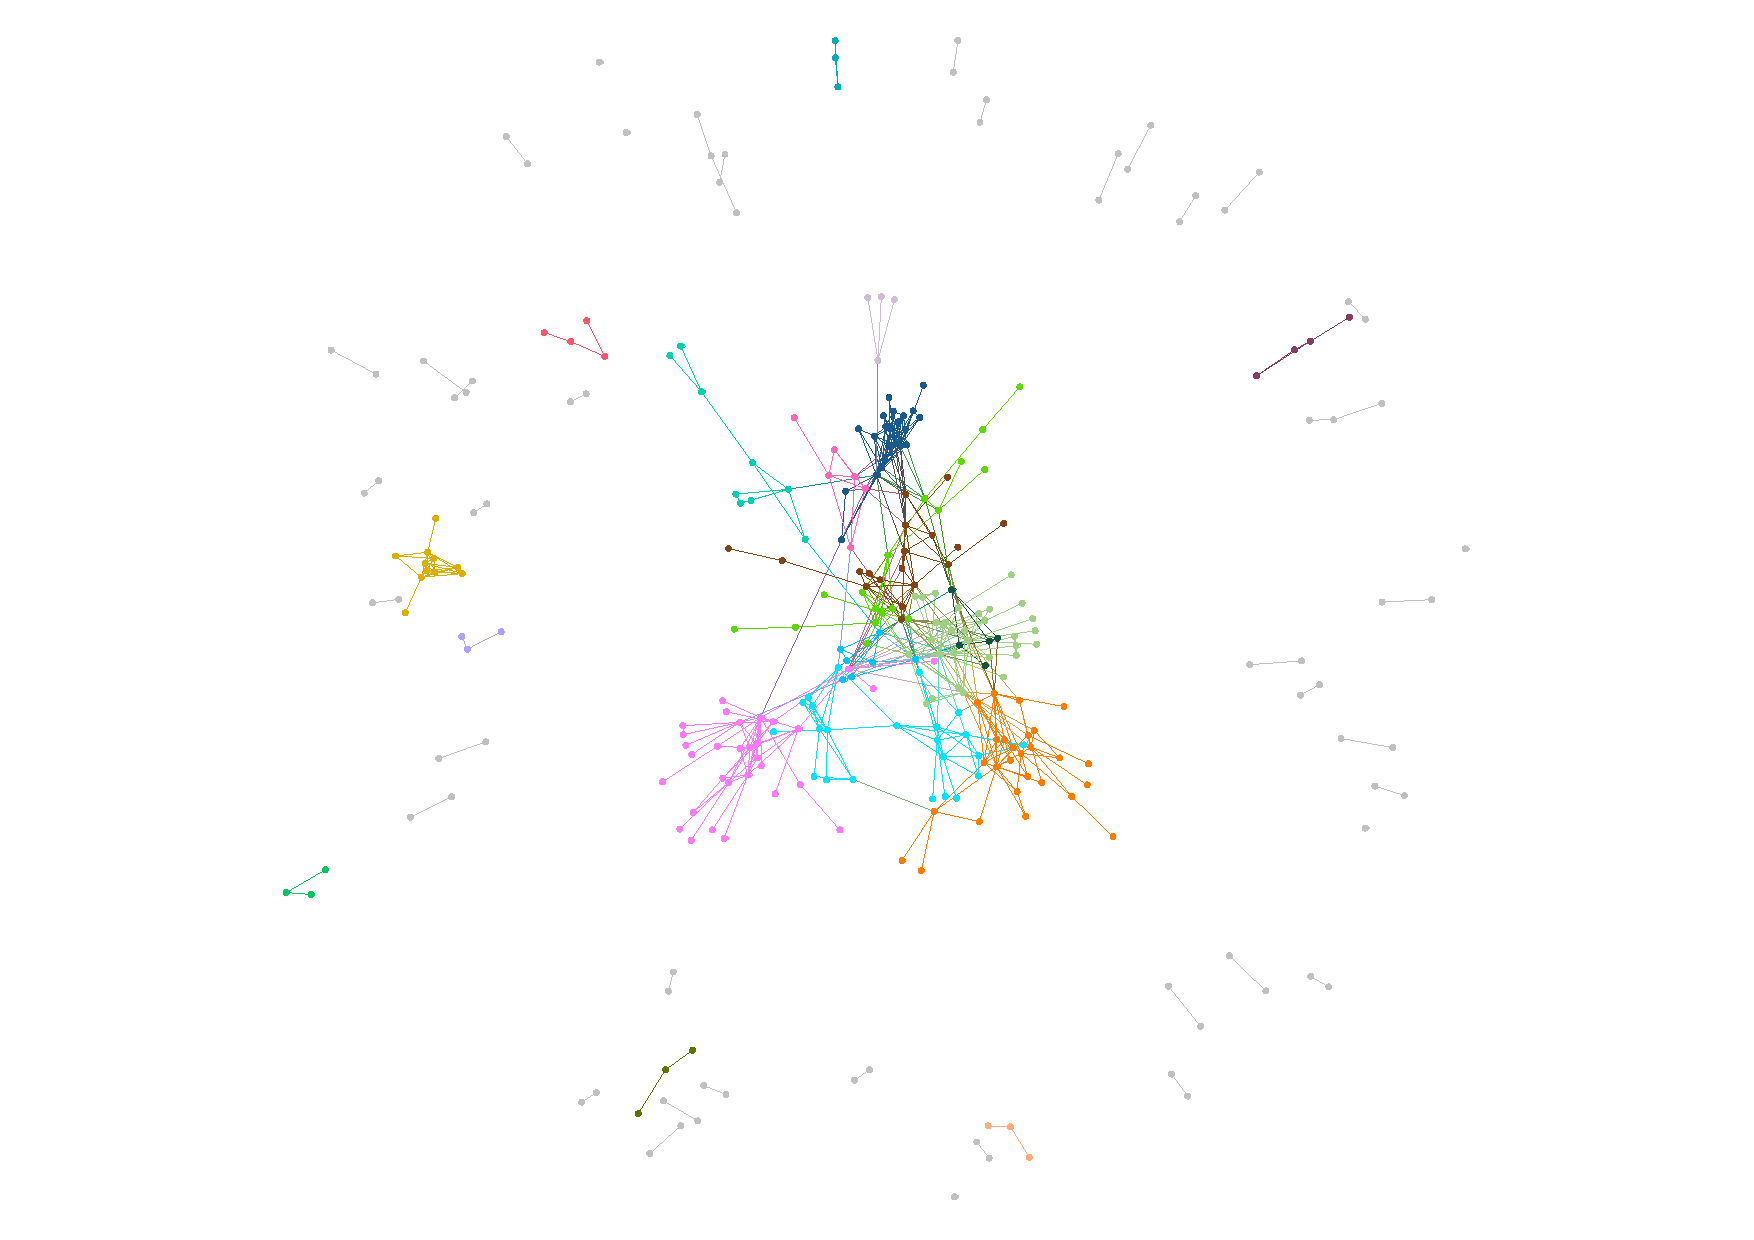
\includegraphics[page=1,scale=0.43]{img/GrafoTuttiEdge.pdf}}
\captionof{figure}{Grafo collaborazioni unificati per coppie di nodi adiacenti}
\label{img:grafotuttiedge}
\end{minipage}
}

\clearpage % grafica da fare alla fine

I nodi del grafo in figura \ref{img:grafopad} si riducono da 306 a 174. Gli edge scendono da 850 a
453, mantenendo il peso totale di 5.195.

\centerline{
\begin{minipage}{1.05\textwidth}
\setlength{\fboxrule}{0pt}	%barbatrucco per far sparire il bordo della box
\fbox{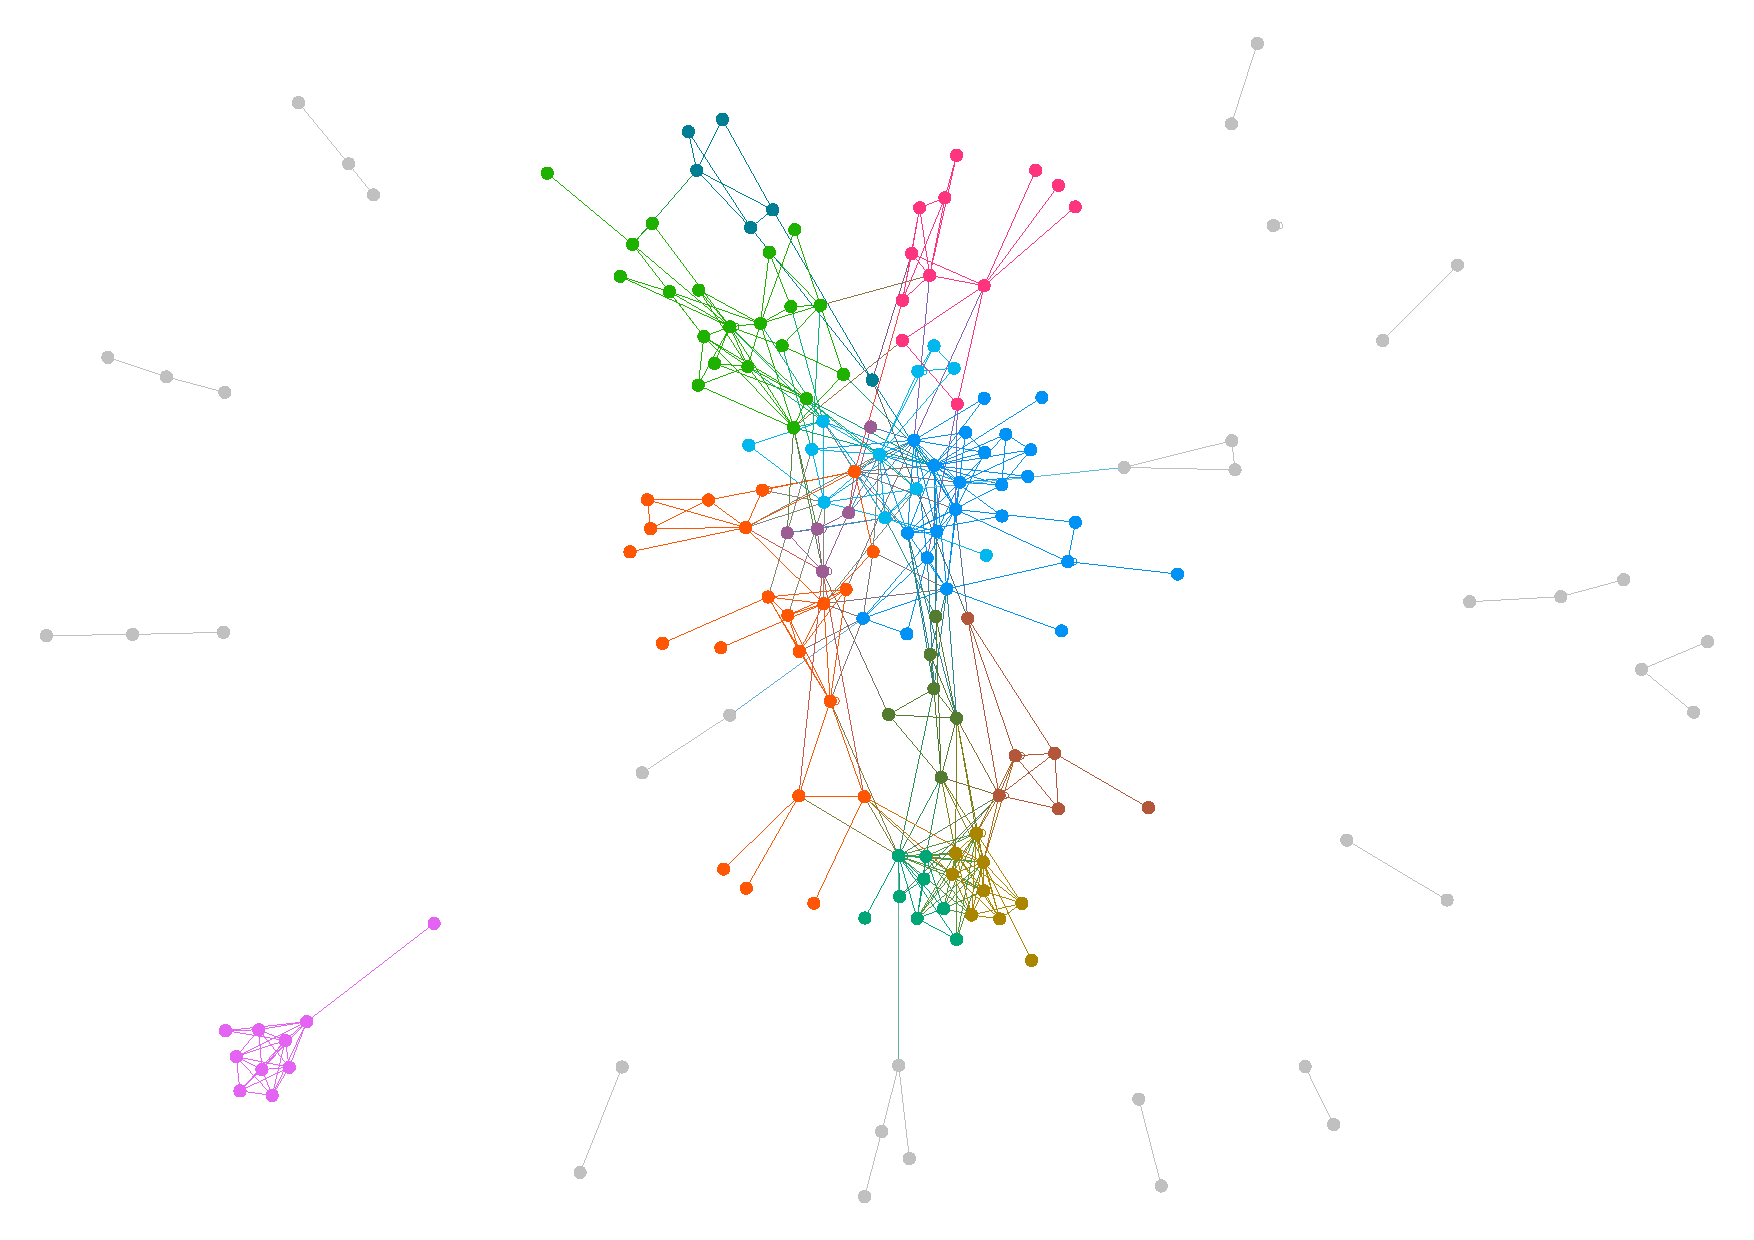
\includegraphics[page=1,scale=0.43]{img/GrafoPadovaniEdge.pdf}}
\captionof{figure}{Grafo Padovani unificati per coppie di nodi adiacenti}
\label{img:grafopadedge}
\end{minipage}
}


\whitePage
\chapter{Troubleshooting} \label{cap:trouble}
Il grafo generato attraverso gli accorgimenti discussi in precedenza presenta ancora delle carenze.

% subsubsection nomi mancanti

La lista di partenza include gli afferenti DEI attuali, mentre il database è aggiornato al 2015.
Questo comporta la mancanza di professori, non più a Padova, che avevano ruolo di aggregatore di una
comunità.

Un metodo proposto per includere i nomi mancanti è:
%estrarre gli ID autore; estrarre i
%paper-aut-aff; da questa lista di paper estrarre tutti gli ID autore; potenzialmente ridurre i paper
%(e gli autori) estratti in base alle affiliation (anche solo del DEI e non di tutta Padova); iterare
%il processo con la nuova lista di autori.
\begin{enumerate}[noitemsep, topsep=0pt]
\item
Estrarre gli ID autore
\item
Estrarre le terne di ID paper-autore-affiliation
\item
Estrarre tutti i record paper-autore-affiliation relativi ai paper identificati al punto precedente
\item
Estrarre una nuova lista di ID autore dai paper appena estratti, ossia i coautori della lista di
partenza.
\item
Eventualmente ridurre il set di autori basandosi sulle affiliation dei loro paper
\item
Ripetere i passi 2-5 per un numero predefinito di volte o fino alla convergenza
\end{enumerate}

In questo modo si estraggono tutte le comunità relative alle affiliation usate come filtro. Una
singola collaborazione con un dipartimento esterno comporta alle iterazioni successive l'inclusione
di molti autori di quel dipartimento. Un metodo proposto per risolvere il problema è, alla fine delle
iterazioni e della creazione dei cluster, considerare solo quelli che contengono almeno un nome
presente nella lista originale: in questo modo dipartimenti esterni, anche se connessi al grafo, non
vengono inclusi.

Per verificare l'efficacia di questo metodo, è stato analizzato il caso del professor Apostolico,
prolifico autore di paper all'Università di Padova, che essendo mancato qualche anno fa non compare
più nella lista degli attuali afferenti al DEI. Dopo aver reinserito il suo nome nella lista di
autori, è stata rieseguita l'estrazione dei dati e rigenerato il grafo.

%Il suo ruolo importante all'interno del suo gruppo di ricerca si nota dalla connessione che
%emerge con i suoi collaboratori, che precedentemente erano distanti nel grafo, come illustrato in
%figura \ref{img:apostolico}
Come illustrato in figura \ref{img:apostolico}, utilizzando questa procedura, emerge una comunità di
collaboratori che precendentemente erano distanti nel grafo.

\centerline{
\begin{minipage}{0.80\textwidth}
\setlength{\fboxrule}{0pt}	%barbatrucco per far sparire il bordo della box
\fbox{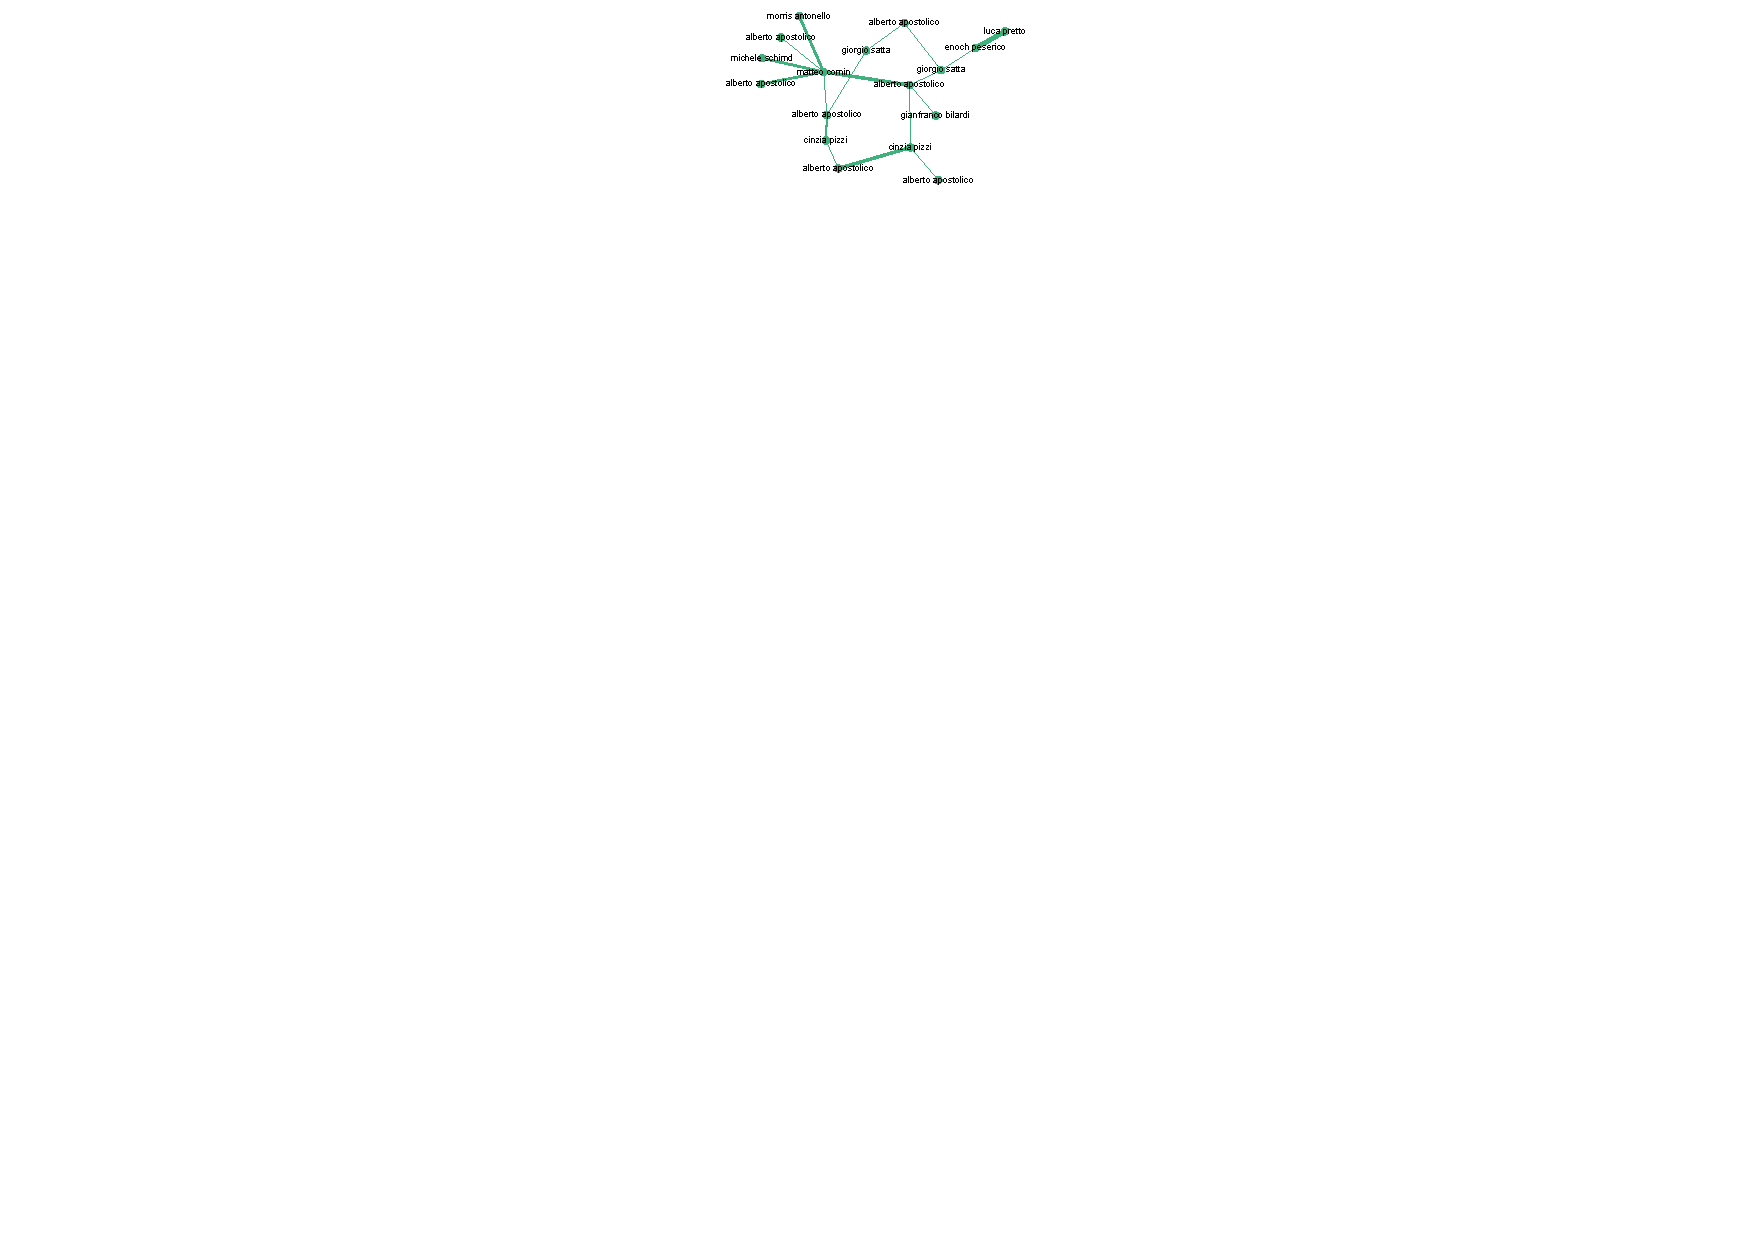
\includegraphics[page=1,scale=1.80]{img/cropped_GrafoApostolico.pdf}}
\captionof{figure}{Rete di collaborazioni del professor Apostolico}
\label{img:apostolico}
\end{minipage}
}

% TODO spiegone amplia rete

% \subsubsection
% TODO scopri cosa fanno i self loop
% TODO mancano proprio record dei paper


\whitePage
\chapter{Risultati} \label{cap:risultati}

\section{V-measure} \label{sec:vmeasure}
Per valutare la qualità delle partizioni dei grafi ricavati con i vari metodi descritti nelle
sezioni precedenti, è stata utilizzata la \textit{V-measure}, come presentata da Rosenberg e
Hirschberg \cite{vmeasure}, una misura esterna della validità dei cluster basata sull'entropia.

Come terminologia, si parlerà di due distinte partizioni del set di nodi del grafo: un set di classi
$C$, considerate la suddivisione reale dei nodi, e un set di cluster $K$ per indicare la partizione
generata.

Rosenberg e Hirschberg hanno sviluppato due concetti, l'omogeneità e la completezza, la cui media
armonica è la V-measure.

Una partizione di cluster è considerata perfettamente omogenea quando i cluster contengono
\textit{solo} membri di una singola classe.

In maniera simmetrica una partizione è perfettamente completa quando un singolo cluster contiene
\textit{tutti} i membri di una classe.

Per valutare l'omogeneità di una partizione si considera l'entropia condizionata della distribuzione
di classi dato il clustering generato $H(C|K)$. Nel caso di perfetta omogeneità questo valore è
nullo, mentre è massimo e vale $H(C)$ quando la distribuzione delle classi all'interno del cluster è
identica alla distribuzione delle classi nell'intero set, per cui il clustering non fornisce alcuna
informazione aggiuntiva. Considerando che il valore di entropia è massimo quando la partizione è
pessima, si definisce l'omogeneità come

\begin{equation} \label{eq:h}
    h = \begin{cases} 1 & \mbox{se } H(C) = 0 \\ 1-\frac{H(C|K)}{H(C)} & \mbox{altrimenti} \end{cases}
\end{equation}

Analogamente si definisce la completezza come

\begin{equation} \label{eq:c}
    c = \begin{cases} 1 & \mbox{se } H(K) = 0 \\ 1-\frac{H(K|C)}{H(K)} & \mbox{altrimenti} \end{cases}
\end{equation}

La \textit{V-measure} è definita come la media armonica pesata dei due valori di omogeneità e
completezza

\begin{equation} \label{eq:c}
    V_\beta = (1+\beta)\frac{h \cdot c}{\beta \cdot h + c}
\end{equation}

Se $\beta<1$ si dà maggior peso all'omogeneità, se $\beta>1$ si dà maggior peso alla completezza. In
questo lavoro è stato usato $\beta=1$

I seguenti diagrammi illustrano graficamente le tre situazioni limite. Le classi sono \{A, B, C,
D\}, i colori rappresentano i cluster.

\begin{center}
\captionof*{table}{Clustering perfetto}
\begin{minipage}{0.30\textwidth}
    \begin{tabular}{|l|r|}
    \hline $h$&1\\
    \hline $c$&1\\
    \hline $V$&1\\
    \hline
    \end{tabular}
\end{minipage}
% \begin{minipage}{0.075\textwidth}
% $\rightarrow$
% \end{minipage}
\begin{minipage}{0.50\textwidth}
    \begin{tikzpicture}
    %\SetGraphUnit{3}
    \GraphInit[vstyle=Normal]
    %\draw[help lines] (0,0) grid (5,3);
    \SetVertexNormal[FillColor=blue!50]
    \Vertex[L=A]{1} % par défaut x = 0 et y = 0
    \Vertex[x=0 , y=3, L=A]{2}
    \Vertex[x=0.5 , y=1.5, L=A]{3}
    \Vertex[x=1.0 , y=0.5, L=A]{4}
    \Vertex[x=1.5 , y=2.5, L=A]{5}
    \SetVertexNormal[FillColor=orange!50]
    \Vertex[x=2.0 , y=1.5, L=B]{6}
    \Vertex[x=2.5 , y=0.0, L=B]{7}
    \Vertex[x=2.5 , y=3.0, L=B]{8}
    \SetVertexNormal[FillColor=red!50]
    \Vertex[x=3.0 , y=1.0, L=C]{9}
    \Vertex[x=3.5 , y=2.0, L=C]{10}
    \SetVertexNormal[FillColor=green!50]
    \Vertex[x=4.0 , y=1.0, L=D]{11}
    \Vertex[x=4.0 , y=3.0, L=D]{12}
    \Vertex[x=5.0 , y=0.5, L=D]{13}
    \Vertex[x=5.0 , y=2.0, L=D]{14}
    \end{tikzpicture}
\end{minipage}
%\medskip
\end{center}
%    \setlength{\abovecaptionskip}{1cm}
\begin{center}
\begin{tabular}{|l|c|c|c|c|c|c|c|c|c|c|c|c|c|c|}
    %\hline ID     &1&2&3&4&5&6&7&8&9&10&11&12&13&14\\
    \hline Classe &A&A&A&A&A&B&B&B&C& C& D& D& D& D\\
    \hline Cluster&1&1&1&1&1&2&2&2&3& 3& 4& 4& 4& 4\\
\hline
\end{tabular}
\end{center}

\begin{center}
\captionof*{table}{Clustering completo ma non omogeneo}
\begin{minipage}{0.30\textwidth}
    \begin{tabular}{|l|r|}
    \hline $h$&0.512\\
    \hline $c$&1\\
    \hline $V$&0.677\\
    \hline
    \end{tabular}
\end{minipage}
\begin{minipage}{0.50\textwidth}
    \begin{tikzpicture}
    \GraphInit[vstyle=Normal]
    %\draw[help lines] (0,0) grid (5,3);
    \SetVertexNormal[FillColor=blue!50]
    \Vertex[L=A]{1} % par défaut x = 0 et y = 0
    \Vertex[x=0 , y=3, L=A]{2}
    \Vertex[x=0.5 , y=1.5, L=A]{3}
    \Vertex[x=1.0 , y=0.5, L=A]{4}
    \Vertex[x=1.5 , y=2.5, L=A]{5}
    \Vertex[x=2.0 , y=1.5, L=B]{6}
    \Vertex[x=2.5 , y=0.0, L=B]{7}
    \Vertex[x=2.5 , y=3.0, L=B]{8}
    \SetVertexNormal[FillColor=orange!50]
    \SetVertexNormal[FillColor=red!50]
    \Vertex[x=3.0 , y=1.0, L=C]{9}
    \Vertex[x=3.5 , y=2.0, L=C]{10}
    \Vertex[x=4.0 , y=1.0, L=D]{11}
    \Vertex[x=4.0 , y=3.0, L=D]{12}
    \Vertex[x=5.0 , y=0.5, L=D]{13}
    \Vertex[x=5.0 , y=2.0, L=D]{14}
    \SetVertexNormal[FillColor=green!50]
    \end{tikzpicture}
\end{minipage}
\end{center}
\begin{center}
\begin{tabular}{|l|c|c|c|c|c|c|c|c|c|c|c|c|c|c|}
    %\hline ID     &1&2&3&4&5&6&7&8&9&10&11&12&13&14\\
    \hline Classe &A&A&A&A&A&B&B&B&C& C& D& D& D& D\\
    \hline Cluster&1&1&1&1&1&1&1&1&2& 2& 2& 2& 2& 2\\
\hline
\end{tabular}
\end{center}

\begin{center}
\captionof*{table}{Clustering omogeneo ma non completo}
\begin{minipage}{0.30\textwidth}
    \begin{tabular}{|l|r|}
    \hline $h$&1\\
    \hline $c$&0.727\\
    \hline $V$&0.842\\
    \hline
    \end{tabular}
\end{minipage}
\begin{minipage}{0.50\textwidth}
    \begin{tikzpicture}
    \GraphInit[vstyle=Normal]
    %\draw[help lines] (0,0) grid (5,3);
    \SetVertexNormal[FillColor=blue!50]
    \Vertex[L=A]{1} % par défaut x = 0 et y = 0
    \Vertex[x=0 , y=3, L=A]{2}
    \Vertex[x=0.5 , y=1.5, L=A]{3}
    \SetVertexNormal[FillColor=orange!50]
    \Vertex[x=1.0 , y=0.5, L=A]{4}
    \Vertex[x=1.5 , y=2.5, L=A]{5}
    \SetVertexNormal[FillColor=red!50]
    \Vertex[x=2.0 , y=1.5, L=B]{6}
    \Vertex[x=2.5 , y=0.0, L=B]{7}
    \Vertex[x=2.5 , y=3.0, L=B]{8}
    \SetVertexNormal[FillColor=green!50]
    \Vertex[x=3.0 , y=1.0, L=C]{9}
    \SetVertexNormal[FillColor=yellow!50]
    \Vertex[x=3.5 , y=2.0, L=C]{10}
    \SetVertexNormal[FillColor=purple!80]
    \Vertex[x=4.0 , y=1.0, L=D]{11}
    \SetVertexNormal[FillColor=gray!50]
    \Vertex[x=4.0 , y=3.0, L=D]{12}
    \Vertex[x=5.0 , y=0.5, L=D]{13}
    \Vertex[x=5.0 , y=2.0, L=D]{14}
    \end{tikzpicture}
\end{minipage}
\end{center}
\begin{center}
\begin{tabular}{|l|c|c|c|c|c|c|c|c|c|c|c|c|c|c|}
    %\hline ID     &1&2&3&4&5&6&7&8&9&10&11&12&13&14\\
    \hline Classe &A&A&A&A&A&B&B&B&C& C& D& D& D& D\\
    \hline Cluster&1&1&1&2&2&3&3&3&4& 5& 6& 7& 7& 7\\
\hline
\end{tabular}
\end{center}
%Preview di due grafici per avere esempi da puntare. Forse punti alla sezione dopo.

\section{Risultati} \label{sec:risultati}

Presentazione dei valori di v-measure per i vari grafi e commenti.

\subsubsection{Tutti vs padovani}\label{ssc:analisitp}
Tra tutti e padovani c'è molta differenza.
\subsubsection{Collassi vari}\label{ssc:analisicollassi}
Tra le varie strade di collasso non c'è sostanziale differenza.
\subsubsection{Metodi di comunity detection}\label{ssc:analisicd}
Tra le varie comunità non c'è sostanziale differenza.

% TODO subsubsection su iterazioni collasso short path e perché non è vero

% TODO alcune strade sono migliori anche se la v-measure è simile

\whitePage
\chapter{Conclusioni} \label{cap:conclusioni}
Partendo da una lista di nomi di un dipartimento si può estrarre un grafo che lo rappresenti? Le comunità generate rispecchiano quelle reali?

TODO se vuoi fallo su matematica e mostra un grafo con qualche valore di v-measure


%%% OBBLIGATORIA:


%::::::::::::::::::::::::::::::::::BIBLIOGRAFIA::::::::::::::::::::::::::::::::::::::::::::::::::::::

% \nocite{*} % visto che non ho citato niente serve per non offendere bibtex
\bibliographystyle{plainurl}
% sarebbe bello usare bibtex ma non funziona, o forse non lo so usare
% vedremo di imparare
\bibliography{tesiautnet} %%% nome file(s)

\end{document}

%::::::::::::::::::::::::::::::::::::::::::::::::::::::::::::::::::::::::::::::::::::::::::::::::::::
